\documentclass[11pt,a4paper,twoside]{report}
\usepackage[a4paper,margin=40mm,headheight=15pt]{geometry}
\usepackage[T1]{fontenc}
\usepackage[utf8]{inputenc}
\usepackage{newtxtext,newtxmath}
\usepackage{microtype}
\usepackage{amsmath,mathtools}
\usepackage{booktabs,longtable,array}
\usepackage{graphicx}
\usepackage{enumitem}
\usepackage{fancyhdr}
\usepackage[numbers,sort&compress]{natbib}
\usepackage[hidelinks]{hyperref}
\hypersetup{pdftitle={Alex Moraru Thesis: Exact Microscopic Reciprocity and Response Rigidity in Chiral Hexagonal Lattice Gases},pdfauthor={Alex Moraru}}
\usepackage[nameinlink,noabbrev]{cleveref}
\usepackage[acronym,toc,nonumberlist]{glossaries}
\usepackage{listings}
\usepackage{xcolor}
\usepackage{caption}
\usepackage{subcaption}
\usepackage{setspace}
\usepackage{siunitx}
\makeglossaries
\newglossaryentry{anchoredcircle}{name={anchored response circle},description={The circle in the complex transport plane with diameter between the origin and the parity symmetric response value. In this work, membership is equivalent to constancy of the real part of the inverse response relative to the anchor}}
\newglossaryentry{chirality}{name={chirality parameter},description={A parameter that changes sign under reflection and measures the bias between opposite handed collision rules. The deterministic HX89 endpoint automata use two discrete chiralities, while the published kinetic model uses a continuous probability parameter}}
\newglossaryentry{collisionoperator}{name={collision operator},description={The local map or its linearized kinetic representation that updates particle occupations during a collision step. Its shear sector determines the kinetic relaxation eigenvalue used in the published molecular chaos calculation}}
\newglossaryentry{commutant}{name={commutant},description={The set of linear maps that commute with a specified symmetry representation. For the real two component shear representation of a nontrivial hexagonal rotation, the commutant is spanned by the identity and a quarter turn matrix}}
\newglossaryentry{defect}{name={circle defect},description={The scalar quantity $\Delta=|Z|^2-x_0\operatorname{Re}Z$ for an anchored response circle. It vanishes exactly on that circle and has a closed expression in terms of the measured inverse response}}
\newglossaryentry{greenkubo}{name={Green Kubo response},description={A transport coefficient or response matrix obtained from an integral of equilibrium or stationary time correlation functions. In two dimensions the limiting procedure requires care because hydrodynamic long time tails can make transport scale dependent}}
\newglossaryentry{hallviscosity}{name={Hall viscosity},description={A parity odd, reactive component of the viscosity tensor, often called odd viscosity. In the two component shear plane it supplies the imaginary coordinate of the complex response used here}}
\newglossaryentry{longtimetail}{name={long time tail},description={An algebraic decay of a hydrodynamic correlation function at late times. Such tails are documented in two dimensional FHP cellular automata and affect how an infinite time Green Kubo limit should be interpreted}}
\newglossaryentry{molecularchaos}{name={molecular chaos},description={A kinetic closure that factorizes precollision correlations so that one particle occupation probabilities determine the collision averages. It enables the published analytical chiral FHP transport coefficients but is not exact for the fully correlated automaton}}
\newglossaryentry{oddviscosity}{name={odd viscosity},description={The antisymmetric part of the viscosity response under exchange of input and output strain indices in a parity broken fluid. It is reactive in the standard constitutive energy balance and is distinct from the dissipative shear viscosity}}
\newglossaryentry{polyform}{name={Polyform},description={The sparse HX89 program representation in which cells are located on a five dimensional integer coordinate field and contain machine operations and operands}}
\newglossaryentry{responsemap}{name={response map},description={The map from a control parameter such as chirality to a point $Z=\bar\eta+i\eta_H$ in the complex transport plane. The geometry of this map is the central object classified in the response rigidity theorem}}
\newglossaryentry{rigidity}{name={response rigidity},description={The condition that the real part of the measured inverse response remains equal to its value at the achiral anchor. For a nonzero complex response, this condition is exactly equivalent to membership in the anchored circle}}
\newglossaryentry{sheardoublet}{name={shear doublet},description={The real two dimensional representation carried by traceless symmetric shear components in two dimensions. A physical rotation through sixty degrees acts on this doublet through twice the angle}}
\newglossaryentry{wardidentity}{name={Ward identity},description={An identity among response functions that follows from a symmetry or conservation law. The circle defect identity derived here is algebraic and is not called a Ward identity because no microscopic conservation law has been shown to enforce the required dissipative flatness}}

\newacronym{crtc}{CRTC}{chiral response transport circle}
\newacronym{fhp}{FHP}{Frisch Hasslacher Pomeau}
\newacronym{gk}{GK}{Green Kubo}
\newacronym{ou}{OU}{Ornstein Uhlenbeck}
\newacronym{rg}{RG}{renormalization group}
\newacronym{c6}{$C_6$}{sixfold rotational symmetry}

% AUTO-GENERATED by thesis/tools/generate_fragments.py. Do not edit.
\newcommand{\HXTransportGridPoints}{3,575}
\newcommand{\HXLocalStates}{64}
\newcommand{\HXGlobalStates}{16,777,216}
\newcommand{\CRTCUnitTests}{35}
\newcommand{\CRTCBoltzmannGridPoints}{9,595}
\newcommand{\CRTCCounterGridPoints}{1,001}
\newcommand{\CRTCCounterOffCircle}{1,000}
\newcommand{\ThesisVerificationDate}{27 September 2026}


\definecolor{codegray}{gray}{0.96}
\lstset{basicstyle=\ttfamily\small,backgroundcolor=\color{codegray},frame=single,breaklines=true,columns=fullflexible,showstringspaces=false}
\pagestyle{fancy}
\fancyhf{}
\fancyhead[LE,LO]{Alex Moraru Thesis}
\fancyhead[RE,RO]{\thepage}
\fancyfoot{}
\renewcommand{\headrulewidth}{0.4pt}
\setcounter{secnumdepth}{3}
\setcounter{tocdepth}{2}
\onehalfspacing
\graphicspath{{figures/}}

\newcommand{\Z}{Z}
\newcommand{\etal}{\textit{et al.}}
\newcommand{\RePart}{\operatorname{Re}}
\newcommand{\ImPart}{\operatorname{Im}}
\newcommand{\e}{\mathrm{e}}
\newcommand{\dd}{\mathrm{d}}

\begin{document}
\begin{titlepage}
\centering
\vspace*{25mm}
{\Large\bfseries Alex Moraru Thesis\par}
\vspace{14mm}
{\huge\bfseries Exact Microscopic Reciprocity and Response Rigidity in Chiral Hexagonal Lattice Gases\par}
\vspace{12mm}
{\Large A structural study of transport circles, inverse response geometry, and correlated counterexamples\par}
\vfill
{\large Alex Moraru\par}
{\large Independent Researcher\par}
\vspace{8mm}
{\large September 2026\par}
\end{titlepage}

\pagenumbering{roman}
\setcounter{page}{1}
\chapter*{Abstract}
\addcontentsline{toc}{chapter}{Abstract}
This thesis studies a narrow structural question in two dimensional chiral transport: when does a pair consisting of dissipative shear viscosity and reactive Hall viscosity lie on an anchored circle as chirality varies, and what survives when molecular chaos is abandoned? The work separates three levels of statement that are often conflated. First, a deterministic six channel hexagonal lattice gas is defined exactly and its microscopic reciprocity properties are proved by operator identities and exhaustive finite state certificates. Second, the published Boltzmann transport coefficients of a chiral Frisch Hasslacher Pomeau model are rewritten as a complex response and shown to obey an exact circle relation. Third, the response geometry is detached from that closure and treated as a theorem about any nonzero complex response.

For a measured response $Z(p)=x(p)+i y(p)$ with a positive parity symmetric anchor $Z(p_0)=x_0$, the anchored circle condition is
\[
 x^2+y^2=x_0x.
\]
The central classification proved here is
\[
 Z(p)\text{ lies on the anchored circle}
 \quad\Longleftrightarrow\quad
 \RePart\!\left[\frac{1}{Z(p)}\right]
 =\RePart\!\left[\frac{1}{Z(p_0)}\right].
\]
If the inverse response is written $Q=a+i b$, the circle defect is exactly
\[
 \Delta=\frac{a_0-a}{a_0(a^2+b^2)}.
\]
Thus reactive drift is compatible with the circle, while dissipative drift is the unique mechanism for leaving this specific anchored circle within the two component response description. Sixfold rotational symmetry is shown to restrict an isolated shear kernel to $aI+bJ$, but it does not force $a$ to be constant. A local curvature formula quantifies quadratic dissipative drift, while an explicit quartic example proves that local curvature at the achiral point is not a complete global classifier.

An analytically solvable stationary Ornstein Uhlenbeck process supplies a correlated Green Kubo counterexample with positive dissipation, reflection covariance, and the same two component symmetry form. Its defect agrees identically with the classification formula. This establishes a nonempty rigid class and a nonempty nonrigid class without tuning data to a circle. It also shows that symmetry and positivity alone do not protect the relation. The remaining physical question is model specific: whether the fully correlated chiral FHP automaton has a renormalized inverse shear response whose real part is chirality independent under a stated finite size, finite time, frequency, or scale prescription. The thesis provides a falsifiable criterion for that question, but does not claim its answer.

\chapter*{Acknowledgments}
\addcontentsline{toc}{chapter}{Acknowledgments}
This work benefited from the published foundations of lattice gas hydrodynamics, linear response theory, and odd viscosity cited throughout the thesis. The computational package was developed so that each central claim can be traced to an executable definition, an exact algebraic check, or a stated external source. Any remaining errors are the responsibility of the author.

\tableofcontents
\listoffigures
\listoftables
\glsaddall
\printglossary[type=\acronymtype,title=List of Abbreviations]
\clearpage
\pagenumbering{arabic}
\setcounter{page}{1}

\chapter{Introduction}\label{ch:introduction}

\section{Question and motivation}
Transport theory usually introduces shear viscosity and Hall viscosity as distinct coefficients with different symmetry properties. The first coefficient multiplies a dissipative shear response. The second is parity odd and reactive in the standard two dimensional constitutive setting \cite{Avron1998,Banerjee2017,FruchartReview2023}. In a microscopic model that breaks parity, both coefficients can depend on the same chirality control parameter. Nothing in their definitions alone requires that dependence to trace a simple geometric curve.

A recent chiral extension of the \gls{fhp} lattice gas provides a useful case. Allocca \etal\ derived closed kinetic expressions for the shear and Hall viscosities and verified their hydrodynamic consequences with cellular automaton simulations \cite{Allocca2026}. At fixed density, those published expressions can be rewritten so that the shifted shear viscosity and Hall viscosity lie exactly on a circle. The circle is therefore not a numerical fit. It is an algebraic consequence of the kinetic formulas.

The natural next question is more difficult. Does the same circle survive when molecular chaos is not assumed and transport is defined from the correlated dynamics? That question matters because two dimensional lattice gases have known hydrodynamic long time correlations \cite{Naitoh1990,ErnstDufty1989}. Correlations can alter dissipative transport, and the limiting value of a zero frequency Green Kubo coefficient can depend on how time, size, and frequency limits are taken. A statement about a renormalized transport circle must therefore be formulated at the level of response structure, not as a request to remove physical correlations from a simulation.

This thesis changes the problem from a direct search for a circle to a classification problem. The object of study is the \gls{responsemap}
\begin{equation}
 Z(p)=\bar\eta(p)+i\eta_H(p),
 \label{eq:intro_response}
\end{equation}
where $p$ is a chirality parameter and $\bar\eta$ denotes the shear coordinate after any explicitly stated lattice shift. The central question is:

\begin{quote}
Which structural property of the inverse response is necessary and sufficient for $Z(p)$ to remain on the parity anchored transport circle, and which admissible response families violate that property?
\end{quote}

This formulation separates geometry from microscopic closure. It can be applied to a kinetic collision matrix, a finite system Green Kubo resolvent, an effective frequency dependent response, or another calculation of the same complex shear sector.

\section{Research questions}
The thesis addresses five linked questions.

\begin{enumerate}[label=\arabic*.]
\item What exact reciprocity statements hold for the deterministic chiral endpoint automata implemented in HX89?
\item How does the published chiral FHP kinetic theory generate a transport circle, and what part of that result is simply complex inversion of a shear eigenvalue?
\item What is the exact, closure independent condition for membership in the anchored response circle?
\item Does sixfold rotational symmetry, reflection covariance, or positive dissipation enforce that condition?
\item What additional information is required before a statement about a collision spectrum becomes a statement about a Green Kubo transport coefficient?
\end{enumerate}

These questions are deliberately ordered from exact microscopic dynamics to response geometry. The order prevents a common logical inversion in which a macroscopic pattern is used to infer a microscopic protection mechanism that has not been proved.

\section{Main results}
The first result is an exact microscopic reciprocity theorem for the deterministic six channel gas used in the repository. Let $C_\chi$ be the local collision permutation at chirality $\chi\in\{-1,+1\}$, let $S$ be toroidal streaming, and let
\begin{equation}
 F_\chi=S C_\chi.
 \label{eq:intro_f}
\end{equation}
With the reflection $P$ and velocity reversal $V$ defined in \cref{ch:microscopic}, the collision dressed involution
\begin{equation}
 \Theta_\chi=C_{-\chi}PV
 \label{eq:intro_theta}
\end{equation}
satisfies
\begin{equation}
 \Theta_\chi^2=I,
 \qquad
 \Theta_\chi F_\chi\Theta_\chi=F_\chi^{-1}.
 \label{eq:intro_reversor}
\end{equation}
Consequently $\Theta_\chi F_\chi^t\Theta_\chi F_\chi^t=I$ for every integer $t$. The local collision table contains \HXLocalStates{} states. The standalone C certificate checks all \HXGlobalStates{} states of the complete $2\times2$ six channel torus for both chiralities, while an independent Python oracle checks larger tori and multiple echo times. These computations verify the finite implementations; the all time statement itself follows from the operator identities.

The second result is a reconstruction of the published molecular chaos transport circle. With
\begin{equation}
 D=\rho\left(1-\frac{\rho}{6}\right)^3,
 \quad
 d=p-\frac12,
 \quad
 A=\frac{1}{2D},
 \quad
 u=\frac{2\sqrt3}{3}d,
 \label{eq:intro_fhp_defs}
\end{equation}
the zero field kinetic coefficients of Allocca \etal\ can be expressed as
\begin{equation}
 \bar\eta=\frac{A}{1+u^2},
 \qquad
 \eta_H=-\frac{Au}{1+u^2}.
 \label{eq:intro_fhp_coeffs}
\end{equation}
Eliminating $u$ gives
\begin{equation}
 \bar\eta^2+\eta_H^2=A\bar\eta.
 \label{eq:intro_boltz_circle}
\end{equation}
The repository checks the zero field identity, its spectral form, and the stated weak field image over \HXTransportGridPoints{} exact rational parameter triples in $\mathbb{Q}(\sqrt3)$. A separate exact grid in the CRTC module checks \CRTCBoltzmannGridPoints{} zero field points. The counts refer to different finite domains and are not combined.

The third result is the response rigidity theorem. Let $Z(p)\ne0$, let the parity symmetric anchor be $p_0$, and assume $Z(p_0)=x_0>0$. Define
\begin{equation}
 \Delta(p)=|Z(p)|^2-x_0\RePart Z(p).
 \label{eq:intro_defect}
\end{equation}
Then
\begin{equation}
 \frac{\Delta(p)}{|Z(p)|^2}
 =1-x_0\RePart\!\left(\frac{1}{Z(p)}\right).
 \label{eq:intro_inverse_identity}
\end{equation}
Since $x_0^{-1}=\RePart[1/Z(p_0)]$, the circle condition $\Delta=0$ is exactly equivalent to
\begin{equation}
 \RePart\!\left(\frac1{Z(p)}\right)
 =\RePart\!\left(\frac1{Z(p_0)}\right).
 \label{eq:intro_rigidity}
\end{equation}
No fixed kinetic prefactor is required. If $1/Z=a+i b$ and $a_0=1/x_0$, then
\begin{equation}
 \Delta=\frac{a_0-a}{a_0(a^2+b^2)}.
 \label{eq:intro_defect_ab}
\end{equation}
This yields a complete two class partition for membership in this specific anchored circle: constant $a$ is the rigid class, while any nonzero drift of $a$ is the nonrigid class. The statement does not classify every possible curve in the response plane, and it does not say that constant curvature by itself is sufficient.

The fourth result identifies what symmetry does and does not supply. The real commutant of the nontrivial $C_6$ action on the two component shear doublet is
\begin{equation}
 M=aI+bJ,
 \qquad
 J=\begin{pmatrix}0&-1\\1&0\end{pmatrix},
 \qquad J^2=-I.
 \label{eq:intro_commutant}
\end{equation}
Reflection makes $a$ even and $b$ odd about the achiral point, but it permits even drift in $a$. Thus $C_6$ symmetry explains the complex scalar form of the response sector, not its rigidity.

The fifth result is an explicit correlated counterexample. A stationary two component Ornstein Uhlenbeck process with drift matrix $K=a(d)I+b(d)J$, covariance $C=AI$, and
\begin{equation}
 a(d)=a_0+\epsilon d^2,
 \qquad
 b(d)=cd,
 \label{eq:intro_ou}
\end{equation}
has positive dissipation for $a_0,\epsilon>0$, an exact Green Kubo integral $R=K^{-1}C$, and a normalized defect
\begin{equation}
 \Delta(d)=
 -\frac{\epsilon d^2}
 {a_0\left[(a_0+\epsilon d^2)^2+c^2d^2\right]}.
 \label{eq:intro_ou_defect}
\end{equation}
It is zero only at the achiral point. The executable exact test evaluates \CRTCCounterGridPoints{} rational points and obtains \CRTCCounterOffCircle{} strict off circle witnesses. A rigid positive dissipation family is obtained by setting $\epsilon=0$. The two classes are therefore both nonempty in a correlated stationary response problem.

\section{Scope of the contribution}
Three boundaries are essential.

First, the deterministic HX89 code implements the endpoint chiralities $\chi=\pm1$. It does not implement the continuous probability $p$ used in the published molecular chaos family. The exhaustive $2^{24}$ certificate therefore proves finite state identities of the endpoint automata; it does not prove a statement for every $p$.

Second, the response rigidity theorem is algebraic. It decides circle membership once the actual complex response $Z$ is known. It does not by itself prove that a particular correlated microscopic model has constant inverse dissipative part.

Third, the defect formula is not presented as a Ward identity. Genuine Ward identities arise from a specified symmetry or conservation law and relate response functions accordingly \cite{Bradlyn2012}. Sixfold rotation gives the normal form in \cref{eq:intro_commutant}, but no conservation law is proved here that forces $a(p)$ to equal its achiral value at every scale.

\section{Organization of the thesis}
\Cref{ch:literature} reviews lattice gas hydrodynamics, Green Kubo transport, odd viscosity, and the published chiral FHP model. \Cref{ch:methodology} defines the evidence hierarchy and reproducibility discipline. \Cref{ch:microscopic} proves the deterministic endpoint reciprocity results. \Cref{ch:kinetic} reconstructs the kinetic transport circle and its spectral form. \Cref{ch:rigidity} proves the closure free classification, the symmetry normal form, and the curvature statements. \Cref{ch:counterexample} constructs the correlated counterexample and analyzes what spectral data can decide. \Cref{ch:discussion} states the remaining Green Kubo problem and its finite regulator formulation. \Cref{ch:conclusion} summarizes what is established and what remains open. The appendices contain proof details, machine definitions, the reproducibility manifest, an adversarial scope audit, and a claim evidence matrix.

\section{Chapter conclusion}
The thesis does not start by assuming that a transport circle survives correlations. It asks what exact property would make survival unavoidable and what admissible dynamics can violate that property. The answer is phrased in the measured inverse response. This provides a strict boundary between an exact structural theorem and the still open correlated chiral FHP question, which is the organizing principle for the chapters that follow.

\chapter{Literature Review}\label{ch:literature}

\section{From lattice gases to hydrodynamics}
The FHP construction established that deterministic Boolean lattice gases on a triangular lattice can reproduce the Navier Stokes equations after coarse graining \cite{FHP1986}. Its importance for the present work is not merely historical. A lattice gas supplies an exactly specified microscopic map, local conservation laws, and finite state dynamics. Those features allow microscopic identities to be checked without floating point ambiguity while still connecting to continuum transport questions.

The separation between exact microdynamics and hydrodynamic closure is already present in the early literature. Poiseuille calculations were used to measure the effective shear viscosity of lattice gas automata and compare the macroscopic flow profile with kinetic predictions \cite{Kadanoff1987}. Green Kubo relations were subsequently derived for lattice gas cellular automata from microscopic conservation laws and correlation functions \cite{ErnstDufty1989}. These results make a useful methodological point: a transport coefficient can be represented through time correlations even when its approximate kinetic value is obtained by a separate molecular chaos closure.

For the present thesis, that distinction is decisive. The deterministic collision and streaming map can obey exact symmetry identities even if the correlated transport coefficient differs from its Boltzmann value. A proof at the level of a collision table therefore does not automatically extend to a proof about a zero frequency Green Kubo viscosity.

\section{Two dimensional correlations and limiting procedures}
Hydrodynamic modes generate algebraic correlation tails in low dimensional fluids. The general language of long wavelength fluctuations and correlation functions is developed in standard treatments such as Forster \cite{Forster1975} and in renormalization analyses of fluid fluctuations \cite{ForsterNelsonStephen1977}. For the two dimensional FHP cellular automaton specifically, Naitoh, Ernst, and Dufty found an intermediate $1/t$ regime in Green Kubo time correlation functions and a later self consistent asymptotic form proportional to $1/[t\sqrt{\ln t}]$ \cite{Naitoh1990}.

This literature rules out a casual instruction to remove long time tails as if they were numerical contamination. They are a physical part of the correlated dynamics. The correct response question must retain a regulator or specify the order of limits. One may use a finite lattice size $L$, a finite integration time $T$, a nonzero frequency $\omega$, or a running coarse graining scale $\ell$. A statement about circle survival can then be asked at fixed regulator before a limiting procedure is attempted.

The distinction also limits what is meant by viscosity in this thesis. The symbol $\eta$ may denote the published kinetic coefficient in \cref{ch:kinetic}, but a fully correlated object should carry its regulator or response prescription when ambiguity is possible. This convention prevents a finite Boltzmann coefficient from being silently identified with an infinite system Green Kubo limit.

\section{Odd viscosity}
Odd viscosity is the parity odd part of the viscosity response and is reactive rather than dissipative in the standard isotropic constitutive decomposition \cite{Avron1998}. In chiral active fluids, broken parity and time reversal can produce such a coefficient in a classical nonequilibrium setting \cite{Banerjee2017}. The broader literature emphasizes that odd transport is compatible with classical stochastic and kinetic models, not only quantum Hall systems \cite{FruchartReview2023}.

Several microscopic approaches are relevant. Fruchart \etal\ used non Hermitian kinetic theory to show how chiral collisions can generate Hall viscosity and odd thermal conductivity \cite{Fruchart2022}. Eren, Fruchart, and Vitelli developed a collisional odd fluid from Boltzmann kinetic theory and related hydrodynamic variables to spectral structure of a linear collision operator \cite{Eren2026}. These works motivate the use of complex eigenvalues and reduced response blocks, but they do not imply the particular anchored circle classified in this thesis.

Green Kubo methods have also been developed and tested for odd viscous fluids. Epstein and Mandadapu derived response relations for two dimensional nonequilibrium viscous fluids with broken time reversal symmetry \cite{Epstein2020}. Hargus \etal\ compared Green Kubo and nonequilibrium molecular dynamics routes for shear and odd viscosity in active fluids \cite{Hargus2020}. The existence of these methods supports the use of a complex correlated response $Z$, but a geometric relation between its real and imaginary parts still requires an additional statement.

\section{Kubo formulas and Ward identities}
Kubo's linear response framework expresses transport through equilibrium or stationary correlation functions \cite{Kubo1957}. For viscosity, care is needed in defining stress response and contact terms. Bradlyn, Goldstein, and Read derived viscosity Kubo formulas from strain generators and analyzed Ward identities that follow from symmetries and, under additional assumptions, relate stress response to conductivity \cite{Bradlyn2012}.

This provides the standard against which any claimed Ward identity should be judged. A Ward identity is not merely a compact algebraic relation. It is tied to a symmetry or conservation law. The response circle identity in this thesis arises from complex inversion and an anchored geometric equation. It becomes Ward like only if a microscopic principle can be found that forces the dissipative inverse response to remain chirality independent. No such principle is established in the present work.

The same caution applies to Kramers Kronig language. Causal analyticity links the real and imaginary parts of a frequency dependent response. The CRTC problem instead follows a control parameter $p$ at fixed response prescription. A geometric relation in the chirality parameter plane is therefore not a nonlinear Kramers Kronig relation. The mathematical resemblance between dissipative and reactive coordinates is not a substitute for the analyticity variable required by the Kramers Kronig construction.

\section{The 2026 chiral FHP model}
Allocca \etal\ introduced parity breaking two body collision rules and a systematic velocity rotation into the FHP framework, derived hydrodynamic transport coefficients, and compared them with Poiseuille flow simulations \cite{Allocca2026}. Their zero field shear sector has a complex relaxation eigenvalue whose real part is independent of the chirality probability $p$ within the molecular chaos calculation. The viscosity pair is an inverse image of that vertical eigenvalue locus.

This observation contains the seed of the response geometry studied here. At fixed density, a vertical line in inverse response space is mapped by complex inversion to a circle through the origin. The circle is therefore a geometric restatement of a specific spectral flatness property in the kinetic model. Once correlations are admitted, the useful question is whether the corresponding real part remains flat after the effective response is computed.

The present thesis relies on the published kinetic formulas as an external premise in \cref{ch:kinetic}. It then reconstructs the algebra independently and checks it exactly over finite rational domains. This is intentionally narrower than claiming the kinetic derivation as original work.

\section{Classical response circles and novelty boundary}
Circular arcs are not new objects in complex response theory. Complex inversion maps generalized circles and lines to generalized circles and lines, and single relaxation response models have long produced semicircular plots. Therefore the novelty claim in this thesis is not that a complex transport coefficient can trace a circle.

The contribution is instead the following combination. First, the chiral FHP kinetic coefficients are placed into a complex inverse response representation with an exact executable reconstruction. Second, the anchored circle is characterized by a necessary and sufficient condition on the measured inverse response that does not require a fixed kinetic prefactor. Third, symmetry is separated from rigidity by an exact commutant calculation. Fourth, a positive dissipation correlated Green Kubo family is constructed that satisfies the symmetry form but violates the circle. Fifth, the role of spectral information is qualified by distinguishing an identified reduced shear block from a bare unordered full spectrum.

This boundary matters because each element answers a different question: prior work supplies the hydrodynamic and transport setting; complex geometry supplies a mathematical mechanism; the present classification identifies the exact invariant that must survive renormalization and provides an explicit witness when it does not.

\section{Chapter conclusion}
The literature supports three premises for the analysis that follows. Deterministic lattice gases can possess exact microscopic structure while their transport is obtained by coarse graining. Two dimensional correlation tails make the fully correlated transport problem nontrivial. Odd viscosity and complex shear response are established concepts, but neither sixfold symmetry nor the existence of a Hall viscosity is known to impose the CRTC circle. These premises motivate an evidence hierarchy that keeps microscopic theorems, kinetic corollaries, and correlated transport conjectures separate.

\chapter{Methodology and Verification Framework}\label{ch:methodology}

\section{Evidence hierarchy}
The computational package is organized around a strict hierarchy of claims. A result is called an exact theorem only when it follows from stated definitions by algebra or finite exhaustive enumeration. A published model corollary is called exact only relative to the cited analytical formulas. A finite parameter sweep is evidence over its declared domain and is never used as a proof over a continuum. A physical statement about the fully correlated chiral FHP transport is called open unless a microscopic or renormalization argument establishes it.

This hierarchy is implemented in \texttt{docs/THEOREM\_STATUS.md} and mirrored in \cref{app:claims}. The purpose is not stylistic. It prevents a verified identity such as $P F_+ P=F_-$ from being rhetorically promoted into a statement about a Green Kubo viscosity, and it prevents a large finite sweep from being described as exhaustive over continuous $p$ or density.

\section{Canonical source of truth}
The thesis is built against the repository tree itself. The machine source, Polyforms, tests, research notes, CRTC module, evidence certificates, scientific registry, and document sources live in one tree. The thesis does not maintain a second manually edited copy of central numerical counts.

The script \texttt{thesis/tools/generate\_fragments.py} reads the transport and chiral certificates, verifies their counts against the declared finite domains in the executable tests, checks the entropy termination cells, counts the current CRTC unit tests, and emits \texttt{thesis/generated/canonical.tex}. The chapter text uses macros from that generated file. Consequently a change in the tested domain makes the generator fail or changes the thesis value in one place rather than leaving stale numbers scattered through prose.

Equation references are handled semantically by LaTeX labels and \texttt{\textbackslash eqref} or \texttt{\textbackslash cref}. Equation numbers are not written by hand in cross references. A changed equation order therefore propagates automatically through the compiled document. The final consistency checker rejects undefined references and citations in the LaTeX log.

\section{Independent implementations}
A useful verification suite should not ask one implementation to certify itself. The repository therefore uses several independent paths.

For the deterministic chiral law, \texttt{src/chiral\_law.c} is a standalone C certificate over the complete $2\times2$ torus, while \texttt{tests/test\_chiral\_law.py} independently implements the collision and streaming logic on larger tori and performs exact rational elimination of one body collision invariants. Agreement between the two paths is stronger evidence against an implementation mistake than repeating one executable with more seeds.

For the transport circle, \texttt{tests/test\_transport\_circle.py} uses exact arithmetic in $\mathbb{Q}(\sqrt3)$ and is separate from the CRTC package. The CRTC module contains its own symbolic and rational tests, including an independently reconstructed $64$ state chiral FHP collision Jacobian.

For the thesis, \texttt{thesis/tools/independent\_math\_audit.py} imports no CRTC implementation. It rederives the inverse response defect, the $C_6$ commutant, the published FHP circle and spectral inversion, the achiral curvature expression, the quartic false negative for local curvature, the Ornstein Uhlenbeck Green Kubo resolvent, and the same spectrum different overlap witness using SymPy from definitions.

\section{Exact arithmetic and finite exhaustive domains}
Floating point tolerances are avoided where exact arithmetic is available. The transport test represents numbers as pairs $(r,s)$ corresponding to $r+s\sqrt3$ with rational $r$ and $s$. This makes the circle and spectral identities exact equalities rather than residual tests.

Two finite domains must be kept distinct. The HX89 transport test evaluates \HXTransportGridPoints{} parameter triples $(\rho,p,B)$, where density assumes eleven half integer values, chirality assumes sixty five rational values, and the weak field parameter assumes five values. The CRTC zero field grid evaluates \CRTCBoltzmannGridPoints{} rational $(\rho,p)$ points on a different domain. Both tests are exhaustive over their declared finite grids. Neither is a continuum proof. The continuum circle identity is instead proved symbolically by eliminating $u$.

The C endpoint certificate is exhaustive in a different sense. A $2\times2$ periodic torus with six Boolean velocity channels per site has $24$ bits and therefore $2^{24}=\HXGlobalStates{}$ states. The program enumerates every state for both endpoint chiralities and verifies the stated reversor and correlation reciprocity identities. The operator proof then extends the echo identity to all integer times on any finite periodic torus because it depends on exact map composition rather than the size of the enumerated example.

\section{Counterexample methodology}
A structural classification is stronger when both sides are inhabited by explicit admissible models. The counterexample in \cref{ch:counterexample} was therefore chosen to satisfy properties that might otherwise be blamed for circle failure: stability, positive symmetric dissipation, a stationary covariance, reflection parity, two component rotational covariance, and an exact Green Kubo integral.

No parameter is adjusted during a run to move a point back to the circle. The arithmetic monitor in the CRTC module may change numerical precision if binary64 inputs overflow, underflow, or collapse distinct decimal values to the same float. It may not change $a$, $b$, $Z$, or the model equations. This boundary is tested explicitly. Numerical recovery is therefore a reliability mechanism, not a physical feedback law.

\section{Software verification}
The repository uses compiler warnings, sanitizer builds, exact tests, and release evidence scripts. The canonical verification workflow includes:
\begin{enumerate}[label=\alph*)]
\item compilation of the assembly and C components;
\item the complete HX89 test suite;
\item AddressSanitizer and UndefinedBehaviorSanitizer runs on the C components;
\item the CRTC symbolic, exact rational, spectral, monitor, and counterexample tests;
\item the independent thesis symbolic audit;
\item generated fragment consistency checks;
\item prose and reference linting;
\item LaTeX compilation with bibliography and glossary generation;
\item PDF render inspection;
\item a final manifest of file hashes.
\end{enumerate}

A passing software suite validates the implementation against its stated assumptions. It does not establish empirical truth beyond those assumptions. In particular, sanitizers can expose memory and undefined behavior defects but cannot prove a hydrodynamic closure.

\section{Reproducibility and external traces}
The evidence tree contains machine generated certificates as well as a set of preserved external CSV traces. The latter are intentionally excluded from proof because their generator, schema, units, ensemble, lattice size, run time, and estimator are not documented. The thesis does not infer missing metadata from column shapes. This is an example of a negative reproducibility rule: unverifiable material may be archived, but it does not support a quantitative claim.

Every central result used positively in the thesis is instead tied to source that can be regenerated locally. The final repository records the verification transcript, environment information supplied by the existing audit, source hashes, and compiled document hashes. \Cref{app:repro} gives the commands and expected certificate lines.

\section{Writing and claim control}
The scientific prose follows the same separation as the code. Terms are defined before use when they are not standard in the immediate context. Present tense is used for mathematical facts and current interpretations, past tense for specific verification runs and cited historical results, and future tense only for proposed work. Promotional adjectives are excluded by a source lint. Unicode dash characters are rejected to avoid typography dependent ambiguities in generated source and rendered documents.

The bibliography is deliberately bounded. A reference is retained when it supplies a foundational result, a directly related transport calculation, a response theory tool, or a specific limitation that affects the argument. The discussion does not use citation density as a substitute for explaining how prior work enters the logic.

\section{Chapter conclusion}
The method of this thesis is recursive in a precise sense: higher level claims are generated from or checked against lower level definitions and certificates, while independent derivations are used to detect self consistent mistakes. The approach cannot guarantee that every physical assumption is correct, but it makes the status and provenance of each claim inspectable. The next chapter applies that discipline to the microscopic chiral automaton before any continuum transport coefficient is introduced.

\chapter{Exact Microscopic Reciprocity in the Deterministic Chiral Gas}\label{ch:microscopic}

\section{Chapter aim}
This chapter establishes the claims that belong entirely to the defined HX89 microscopic objects. No viscosity coefficient is used. The purpose is to isolate what can be proved from the collision table, streaming map, reflection, and velocity reversal before any kinetic closure is introduced.

\section{State space and collision map}
Each lattice site carries six Boolean occupations, one for each velocity direction of the hexagonal lattice. A local state is therefore an integer in $\{0,\ldots,63\}$ or, equivalently, a vector in $\{0,1\}^6$. The deterministic chirality variable is
\begin{equation}
 \chi\in\{-1,+1\}.
 \label{eq:chi_endpoint}
\end{equation}
The two endpoint collision maps are permutations. In the positive chirality convention the nontrivial two particle pair cycle is
\begin{equation}
 9\mapsto18\mapsto36\mapsto9,
 \label{eq:pair_cycle}
\end{equation}
and the complementary three particle pair is exchanged,
\begin{equation}
 21\leftrightarrow42.
 \label{eq:triple_swap}
\end{equation}
All other local states are fixed by the chiral component of the table. The negative chirality collision is the inverse permutation,
\begin{equation}
 C_{-}=C_{+}^{-1}.
 \label{eq:collision_inverse}
\end{equation}
The precise executable definition is in \texttt{src/chiral\_law.c}; the description here records the algebraic structure rather than replacing the source.

A full time step first applies the local collision at every site and then streams each occupied velocity channel to the neighboring site indicated by its velocity. On a finite periodic axial torus,
\begin{equation}
 F_\chi=S C_\chi.
 \label{eq:full_step}
\end{equation}
Both $C_\chi$ and $S$ are bijections, hence $F_\chi$ is a bijection of the finite configuration space.

\section{Reflection and velocity reversal}
Let $P$ denote the axial reflection implemented by the reference oracle. In axial lattice coordinates it acts on position as
\begin{equation}
 P:(x,y)\mapsto(x+y,-y),
 \label{eq:axial_reflection}
\end{equation}
and it reverses the angular index of the velocity channel. Let $V$ be velocity reversal,
\begin{equation}
 V:i\mapsto i+3\pmod 6.
 \label{eq:velocity_reversal}
\end{equation}
Both maps are involutions. Direct examination of the local table gives the mirror chirality relation
\begin{equation}
 P C_{+} P=C_{-},
 \label{eq:collision_mirror}
\end{equation}
while spatial reflection conjugates streaming into the reflected streaming map in the corresponding channel coordinates.

The naive composition $PV$ does not by itself provide the required reversor for the collision then streaming ordering. The collision order matters. The exact involution is collision dressed.

\section{Collision dressed reversor}
Define
\begin{equation}
 \Theta_\chi=C_{-\chi}PV.
 \label{eq:theta_def}
\end{equation}
The local permutation identities and the relation between streaming and velocity reversal imply
\begin{equation}
 \Theta_\chi^2=I
 \label{eq:theta_involution}
\end{equation}
and
\begin{equation}
 \Theta_\chi F_\chi\Theta_\chi=F_\chi^{-1}.
 \label{eq:theta_reversor}
\end{equation}
The proof is a composition proof. It does not rely on sampling trajectories. Once \cref{eq:theta_involution,eq:theta_reversor} hold, induction gives
\begin{equation}
 \Theta_\chi F_\chi^t\Theta_\chi=F_\chi^{-t}
 \label{eq:theta_time}
\end{equation}
for every integer $t$, and therefore
\begin{equation}
 \Theta_\chi F_\chi^t\Theta_\chi F_\chi^t=I.
 \label{eq:echo_identity}
\end{equation}
The last identity is the exact echo theorem used by the executable tests.

This result is sometimes easy to misdescribe. It is not ordinary time reversal under $V$ alone, and it does not assert detailed balance for a stochastic transition matrix. It is a deterministic reversor identity for the stated endpoint map. The collision dressing is essential because the forward map is ordered as collision followed by streaming.

\section{Reflection and chirality reciprocity}
Reflection changes chirality. At the full map level the implemented identities imply
\begin{equation}
 P F_{+} P=F_{-}
 \label{eq:full_mirror}
\end{equation}
with the coordinate conventions of the executable oracle. If an ensemble measure is invariant under the relevant reflected mapping and observables have definite parity, correlation functions inherit a reciprocity relation between the two chiralities. The repository verifies a finite correlation witness in the exhaustive C certificate and checks the general map identities independently in Python.

This distinction between map reciprocity and ensemble reciprocity is important. The first is an identity of deterministic maps. The second also depends on how configurations are weighted. A correlation identity should therefore state its measure assumptions explicitly rather than treating them as automatic consequences of the collision permutation.

\section{One body collision invariants}
The collision table conserves particle number and the two components of lattice momentum. The independent Python oracle constructs the linear system for all one body quantities
\begin{equation}
 I(n)=\sum_{i=0}^{5}c_i n_i
 \label{eq:onebody_general}
\end{equation}
that are unchanged by every local collision. Exact rational row reduction yields a three dimensional invariant space. A basis can be chosen as total occupation and the two momentum components.

This is stronger than checking several expected invariants and weaker than classifying every possible nonlinear invariant. It states exactly that the vector space of one body linear collision invariants for the implemented local table has rank three.

\section{Exhaustive finite state certificate}
The standalone program \texttt{bin/hx89-chiral-proof} constructs the complete periodic $2\times2$ lattice. Four sites with six Boolean channels produce $24$ bits and therefore
\begin{equation}
 2^{24}=\HXGlobalStates{}
 \label{eq:global_state_count}
\end{equation}
configurations. The certificate enumerates all of them for both endpoint chiralities and checks the mirror chirality relation, the involution property, the dressed reversor, the echo, and a correlation reciprocity witness. The local collision table separately contains \HXLocalStates{} states.

The present evidence file records the certificate line
\begin{quote}\ttfamily
CHIRAL\_LAW\_PASS local\_states=64 global\_states=16777216 mirror\_chirality=PASS theta\_involution=PASS dressed\_PT\_reversor=PASS echo=PASS correlation\_reciprocity=PASS both\_chiralities=PASS
\end{quote}
The full line, including exact correlation numerators and denominators, is preserved in \texttt{evidence/chiral\_law\_certificate.txt} rather than duplicated as a manually maintained number in the prose.

Exhausting a $2\times2$ torus does not by itself prove an identity on every lattice size. Here the finite exhaustive certificate serves as an implementation witness for the local and composed maps. The size independent theorem comes from the operator identities in \cref{eq:theta_involution,eq:theta_reversor}. The independent larger torus oracle is a further check that the implementation of those identities is not accidentally tied to the enumerated lattice.

\section{Entropy Polyform termination regression}
The repository also contains a five dimensional sparse Polyform example in which an entropy instruction chooses one of ten signed spatial directions from the origin. A previous failure mode occurred when the emitted branch advanced into a coordinate with no defined sparse cell. For seed $12345$ the branch selected the fifth positive axis, emitted its axis letter, and advanced to $(0,0,0,0,2)$.

The corrected program defines an explicit zero opcode HALT cell at each of the ten signed distance two endpoints. The regression test checks seed $12345$ and then covers all ten direction and sign outcomes. The semantic point is narrow but useful: intentional termination is represented by an actual cell, while a genuinely missing sparse cell remains an error. The runtime is not changed to suppress out of bounds execution globally.

This regression is not part of the chiral fluid theorem. It is included in the same verification tree because the user facing repository combines the machine framework and the transport research. The thesis treats it as engineering evidence, not physics evidence.

\section{What the microscopic theorem does not imply}
Three deductions are explicitly excluded.

First, the endpoint theorem does not generate the continuous probability parameter $p$ used by the chiral FHP molecular chaos model. A deterministic map at $\chi=\pm1$ is not an exhaustive sample of a stochastic or mixed collision family.

Second, the reversor does not force a specific value of a viscosity. Transport coefficients depend on correlation functions and projections onto hydrodynamic sectors. Exact reversibility can constrain those correlations without fixing the real part of the inverse shear response as chirality changes.

Third, the finite state certificate does not remove long time hydrodynamic effects. A finite deterministic automaton is periodic at sufficiently long time because its configuration space is finite, while a hydrodynamic limit concerns a scaling regime of size and time. Those are different mathematical statements.

\section{Chapter conclusion}
The deterministic endpoint gas has an exact collision dressed reversor, mirror chirality reciprocity, and precisely three one body linear collision invariants. These results are established independently of any transport closure. They provide a controlled microscopic foundation for discussing chirality, but they do not prove a transport circle. The next chapter introduces the published continuous chiral FHP kinetic theory and shows exactly where its circle comes from.

\chapter{The Molecular Chaos Transport Circle}\label{ch:kinetic}

\section{Chapter aim and attribution}
This chapter reconstructs a geometric consequence of the analytical transport coefficients derived by Allocca \etal\ for a chiral FHP cellular automaton \cite{Allocca2026}. The continuum coefficients and the underlying kinetic derivation are attributed to that work. The contribution here is the exact elimination, spectral rewriting, independent finite arithmetic verification, and the separation between that kinetic identity and the correlated problem studied later.

\section{Parameterization of the published coefficients}
Let $\rho$ be the mean occupancy density and let $p$ denote the probability that resolves the chiral collision choice in the published model. Introduce
\begin{equation}
 d=p-\frac12,
 \qquad
 D=\rho\left(1-\frac{\rho}{6}\right)^3.
 \label{eq:kin_D}
\end{equation}
Away from the singular endpoints $D=0$, define
\begin{equation}
 A=\frac{1}{2D},
 \qquad
 u=\frac{2\sqrt3}{3}d.
 \label{eq:kin_Au}
\end{equation}
The lattice contribution is most conveniently absorbed into the shifted shear coordinate
\begin{equation}
 \bar\eta=\eta+\frac18.
 \label{eq:eta_shift}
\end{equation}
The zero field transport formulas can then be written
\begin{equation}
 \bar\eta=\frac{A}{1+u^2},
 \qquad
 \eta_H=-\frac{Au}{1+u^2}.
 \label{eq:kin_coeffs}
\end{equation}
The parity symmetric point is $p=1/2$, where $u=0$ and $\eta_H=0$.

\section{Elimination of chirality}
Squaring the two expressions in \cref{eq:kin_coeffs} gives
\begin{align}
 \bar\eta^2+\eta_H^2
 &=\frac{A^2(1+u^2)}{(1+u^2)^2}\\
 &=\frac{A^2}{1+u^2}\\
 &=A\bar\eta.
 \label{eq:kin_circle_shifted}
\end{align}
Completing the square yields
\begin{equation}
 \left(\bar\eta-\frac{A}{2}\right)^2+\eta_H^2
 =\left(\frac{A}{2}\right)^2.
 \label{eq:kin_circle_centered}
\end{equation}
Returning to the unshifted coordinate,
\begin{equation}
 \left(\eta+\frac18-\frac{A}{2}\right)^2+\eta_H^2
 =\left(\frac{A}{2}\right)^2.
 \label{eq:kin_circle_eta}
\end{equation}
At each fixed density the kinetic response therefore lies on an arc of a circle in the $(\eta,\eta_H)$ plane. The radius and center depend on density through $A$. The curve traversed by $p\in[0,1]$ need not cover the whole circle.

\begin{figure}[htbp]
\centering
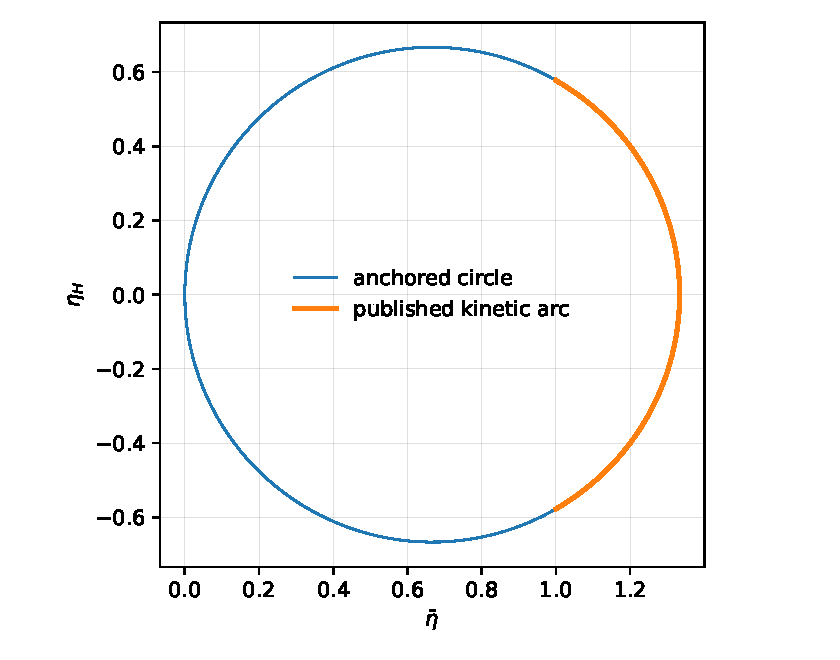
\includegraphics[width=.72\textwidth]{fhp_transport_circle.pdf}
\caption{Analytic molecular chaos response arc at $\rho=3$, generated directly from \cref{eq:kin_coeffs}. The thin curve is the complete anchored circle from \cref{eq:kin_circle_centered}; the thicker curve is the interval traced by $p\in[0,1]$. This is an analytic figure, not simulation data.}
\label{fig:fhp_circle}
\end{figure}

\section{Complex spectral form}
The same geometry is more informative when written as a complex response
\begin{equation}
 Z_B=\bar\eta+i\eta_H.
 \label{eq:zb_def}
\end{equation}
The shear sector eigenvalue of the published molecular chaos collision matrix can be written in the conventions used by the test suite as
\begin{equation}
 \lambda=-\frac{D}{2}+i\frac{\sqrt3 D}{3}d.
 \label{eq:kin_lambda}
\end{equation}
Direct inversion gives
\begin{equation}
 Z_B=-\frac{1}{4\lambda^*}.
 \label{eq:kin_spectral}
\end{equation}
The real part of $\lambda$ is $-D/2$ and is independent of $p$ at fixed density. As $p$ varies, $\lambda$ therefore moves on a vertical line in the complex plane. Conjugation and multiplication by a nonzero scalar preserve the line structure, and complex inversion maps a line not through the origin to a circle through the origin. The transport circle is thus the inverse image of dissipative spectral flatness in this kinetic model.

This observation is stronger conceptually than the completed square. It identifies which part of the eigenvalue produces the circle. The imaginary part carries the chirality dependent reactive coordinate. The fixed real part sets the circle. If correlations renormalize only the imaginary part of the effective inverse response, the circle survives. If they introduce chirality dependence into the real part, the anchored circle is broken.

\section{Exact finite verification in $\mathbb{Q}(\sqrt3)$}
The test \texttt{tests/test\_transport\_circle.py} avoids floating point arithmetic. Every quantity is represented as $r+s\sqrt3$ with rational $r$ and $s$. The test evaluates eleven density values, sixty five chirality values, and five weak field values, for a total of
\begin{equation}
 \HXTransportGridPoints{}
 \label{eq:transport_grid_count}
\end{equation}
parameter triples. At every point it checks the zero field circle, \cref{eq:kin_spectral}, and the stated weak field transformed circle exactly.

The CRTC package contains a separate zero field grid. It evaluates densities $\rho=n/16$ for $n=1,\ldots,95$ and chirality values $p=m/100$ for $m=0,\ldots,100$. This gives
\begin{equation}
 95\times101=\CRTCBoltzmannGridPoints{}
 \label{eq:crtc_boltz_grid_count}
\end{equation}
exact rational points. The test checks the polynomial circle identity at every point. The two counts are not alternative reports of the same run. They cover different finite parameter sets and test overlapping but not identical statements.

These finite checks do not prove the continuum relation. The proof is the algebra in \cref{eq:kin_circle_shifted}. Their role is to verify that the executable formulas, sign conventions, lattice shift, field transformation, and spectral relation agree with the symbolic derivation across broad finite domains.

\section{Weak field transformation}
The HX89 transport test also implements the weak field image given in the cited model. In the test conventions, with $b=B/2$ and scale $1+b^2$, the pair $(\eta,\eta_H)$ is transformed by a scaled rotation. The lattice shift must be carried through the same complex factor. Once that shift is handled consistently, the image of the zero field circle is again a circle with the correspondingly transformed center and radius.

The point of this test is bookkeeping as much as physics. A coordinate shift that is applied to shear viscosity at zero field but forgotten after a complex rotation can create a spurious circle defect. Exact arithmetic makes such a mismatch visible immediately. The thesis therefore treats the shifted coordinate $\bar\eta$ as part of the response definition whenever the Boltzmann formula is used.

\section{Relation to the inverse response classifier}
The kinetic circle can be put directly into the closure free language developed in \cref{ch:rigidity}. From \cref{eq:kin_spectral},
\begin{equation}
 \frac{1}{Z_B}=-4\lambda^*.
 \label{eq:kin_inverse_z}
\end{equation}
Hence
\begin{equation}
 \RePart\!\left(\frac{1}{Z_B}\right)=2D,
 \label{eq:kin_inverse_real}
\end{equation}
which is independent of $p$ at fixed density. The published kinetic circle is therefore a direct instance of inverse response rigidity.

This formulation also shows why a fixed prefactor should not be treated as fundamental. If one writes $Z=A_1/(\alpha+i\beta)$ with a parameter dependent residue $A_1(p)$, it is the ratio $\alpha/A_1$ that appears in the measured inverse response. The classifier should be applied to $1/Z$ itself. It does not require an assumption that a kinetic overlap or susceptibility prefactor remains unrenormalized.

\section{What this chapter proves}
The chapter proves three statements conditional only on the cited kinetic formulas:
\begin{enumerate}[label=\alph*)]
\item eliminating the chirality parameter produces the circle \cref{eq:kin_circle_eta};
\item the complex response is the inverse of the conjugate shear eigenvalue up to the stated factor, \cref{eq:kin_spectral};
\item the finite executable representations agree with those identities over their declared exact domains.
\end{enumerate}

It does not prove that the fully correlated automaton has the same transport coefficients. Molecular chaos enters before \cref{eq:kin_coeffs}; algebra performed afterward cannot remove that premise. The distinction becomes central in \cref{ch:discussion}.

\section{Chapter conclusion}
The published chiral FHP kinetic transport circle is an exact geometric image of a vertically flat shear eigenvalue locus. This gives a concrete model in which dissipative flatness and reactive chirality produce a circle by complex inversion. The result suggests the correct structural variable for a correlated theory: not the raw shear and Hall viscosities separately, but the real part of their measured inverse complex response. The next chapter proves that this observation is in fact an exact equivalence for any nonzero response, independent of the kinetic closure.

\chapter{Response Rigidity, Symmetry, and Curvature}\label{ch:rigidity}

\section{Anchored response geometry}
Let $p$ vary in an interval containing a parity symmetric point $p_0$. Let
\begin{equation}
 Z(p)=x(p)+iy(p)\ne0
 \label{eq:rig_z}
\end{equation}
be the measured complex shear response under a fixed response prescription. Assume the anchor is real and positive,
\begin{equation}
 Z(p_0)=x_0>0.
 \label{eq:rig_anchor}
\end{equation}
The circle whose diameter joins $0$ to $x_0$ on the real axis has equation
\begin{equation}
 \left(x-\frac{x_0}{2}\right)^2+y^2
 =\left(\frac{x_0}{2}\right)^2.
 \label{eq:rig_circle_center}
\end{equation}
Equivalently,
\begin{equation}
 x^2+y^2=x_0x.
 \label{eq:rig_circle}
\end{equation}
Define the signed algebraic defect
\begin{equation}
 \Delta(p)=|Z(p)|^2-x_0\RePart Z(p).
 \label{eq:rig_delta}
\end{equation}
Circle membership is exactly the zero set $\Delta=0$.

\section{Closure free classification theorem}
Since $Z\ne0$,
\begin{equation}
 \RePart\!\left(\frac1Z\right)
 =\frac{\RePart Z}{|Z|^2}.
 \label{eq:rig_inverse_real}
\end{equation}
Divide \cref{eq:rig_delta} by $|Z|^2$ to obtain
\begin{equation}
 \frac{\Delta}{|Z|^2}
 =1-x_0\RePart\!\left(\frac1Z\right).
 \label{eq:rig_master_identity}
\end{equation}
At the anchor, $1/Z(p_0)=1/x_0$. Therefore:

\paragraph{Response rigidity theorem.}
For every nonzero complex response satisfying \cref{eq:rig_anchor},
\begin{equation}
 \Delta(p)=0
 \quad\Longleftrightarrow\quad
 \RePart\!\left(\frac1{Z(p)}\right)
 =\RePart\!\left(\frac1{Z(p_0)}\right).
 \label{eq:rig_theorem}
\end{equation}

The proof is the identity \cref{eq:rig_master_identity}. No simulation, kinetic closure, collision model, or fixed response prefactor is required. The theorem classifies membership in one specified anchored circle. It does not say that every curve of constant curvature is this circle, nor that every generalized circle must pass through the anchor and origin.

\begin{figure}[htbp]
\centering
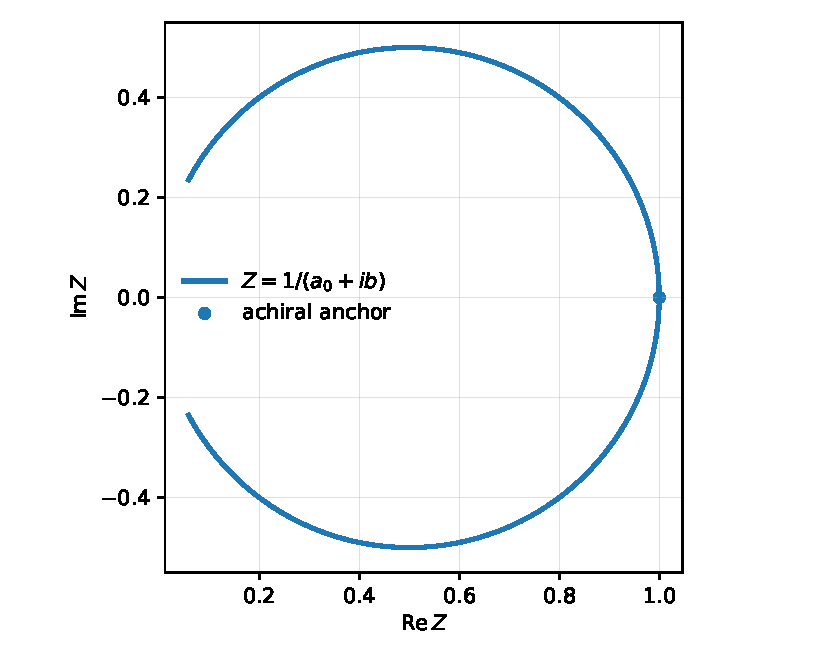
\includegraphics[width=.72\textwidth]{inverse_response_geometry.pdf}
\caption{Complex inversion of the vertical inverse response locus $\RePart(1/Z)=a_0$ produces the anchored circle. The plotted curve uses $a_0=1$ and is generated analytically from $Z=1/(a_0+i b)$.}
\label{fig:inverse_geometry}
\end{figure}

\section{Kernel coordinates and the defect formula}
Write the measured inverse response as
\begin{equation}
 Q(p)=\frac1{Z(p)}=a(p)+ib(p),
 \label{eq:q_ab}
\end{equation}
and define
\begin{equation}
 a_0=a(p_0)=\frac1{x_0}.
 \label{eq:a0}
\end{equation}
Then
\begin{equation}
 Z=\frac{a-ib}{a^2+b^2},
 \qquad
 |Z|^2=\frac{1}{a^2+b^2}.
 \label{eq:z_ab}
\end{equation}
Substitution into \cref{eq:rig_delta} gives
\begin{equation}
 \boxed{
 \Delta(p)=\frac{a_0-a(p)}{a_0\left[a(p)^2+b(p)^2\right]}}
 \label{eq:defect_ab}
\end{equation}
for the normalized measured response.

Several consequences follow immediately. Arbitrary changes of the reactive coordinate $b(p)$ preserve the circle if $a(p)=a_0$. Any drift of $a$ away from $a_0$ produces a nonzero defect. Within this two coordinate description there is no third class for the membership predicate: a point is either on the anchored circle because the inverse real part equals $a_0$, or it is off that circle because the inverse real part differs.

If a model is instead parameterized as
\begin{equation}
 Z(p)=\frac{A(p)}{\alpha(p)+i\beta(p)},
 \label{eq:prefactor_model}
\end{equation}
then
\begin{equation}
 \RePart\!\left(\frac1Z\right)=\frac{\alpha(p)}{A(p)}.
 \label{eq:prefactor_ratio}
\end{equation}
It is therefore not correct in general to identify rigidity with constant $\alpha$ alone. The closure free theorem is written in terms of the actual measured $1/Z$ precisely to absorb any response residue or normalization into the observable quantity.

\section{Sixfold symmetry and the shear commutant}
The traceless symmetric shear components in two dimensions form a real two component representation. A physical rotation through angle $\theta$ acts on this doublet through angle $2\theta$. For a nontrivial element of $C_6$, one may use the $120$ degree matrix
\begin{equation}
 R=\begin{pmatrix}
 -\tfrac12&-\tfrac{\sqrt3}{2}\\
 \tfrac{\sqrt3}{2}&-\tfrac12
 \end{pmatrix}.
 \label{eq:c6_rotation}
\end{equation}
Let
\begin{equation}
 M=\begin{pmatrix}m_{11}&m_{12}\\m_{21}&m_{22}\end{pmatrix}
 \label{eq:generic_m}
\end{equation}
be a real linear operator that commutes with $R$. Solving $MR=RM$ gives
\begin{equation}
 m_{11}=m_{22},
 \qquad
 m_{12}=-m_{21}.
 \label{eq:commutant_constraints}
\end{equation}
Thus
\begin{equation}
 M=aI+bJ,
 \qquad
 J=\begin{pmatrix}0&-1\\1&0\end{pmatrix}.
 \label{eq:commutant_form}
\end{equation}
The independent symbolic audit solves this commutator equation directly and verifies that the commutant is two dimensional.

Reflection conjugates $J$ to $-J$. If chirality displacement $d=p-p_0$ changes sign under reflection, covariance implies the parity structure
\begin{equation}
 a(d)=a(-d),
 \qquad
 b(d)=-b(-d).
 \label{eq:parity_ab}
\end{equation}
This is not enough to make $a$ constant. Terms such as $a_2d^2$, $a_4d^4$, and higher even powers are symmetry allowed. Sixfold symmetry gives the complex scalar form, while rigidity is an additional condition.

\section{Curvature of the response map}
The response map is a plane curve $r(d)=(x(d),y(d))$. Its signed curvature for a regular parameterization is
\begin{equation}
 \kappa(d)=
 \frac{x'(d)y''(d)-y'(d)x''(d)}
 {\left[x'(d)^2+y'(d)^2\right]^{3/2}}.
 \label{eq:curvature_general}
\end{equation}
Assume parity near $d=0$ and expand
\begin{equation}
 a(d)=a_0+\frac{a_2}{2}d^2+O(d^4),
 \qquad
 b(d)=b_1d+O(d^3),
 \label{eq:local_expansion}
\end{equation}
with $b_1>0$ setting the orientation. Substituting $Z=1/(a+ib)$ into \cref{eq:curvature_general} gives
\begin{equation}
 \boxed{
 \kappa(0)=-2a_0-\frac{a_0^2a_2}{b_1^2}}
 \label{eq:curvature_achiral}
\end{equation}
for the chosen orientation convention. In the rigid class $a_2=0$ and the anchored circle has radius $1/(2a_0)$, so its signed curvature is $-2a_0$.

Equation \cref{eq:curvature_achiral} makes the role of quadratic dissipative drift concrete. It also explains why curvature is useful as a local diagnostic. If $a_2\ne0$, the achiral curvature differs from the rigid circle value.

\section{Why local curvature is not a global classifier}
Curvature at one point cannot decide global circle membership. Consider
\begin{equation}
 a(d)=a_0+\epsilon d^4,
 \qquad
 b(d)=cd.
 \label{eq:quartic_drift}
\end{equation}
Then $a''(0)=0$, so \cref{eq:curvature_achiral} gives the same achiral curvature as the rigid circle. Nevertheless \cref{eq:defect_ab} becomes
\begin{equation}
 \Delta(d)=
 -\frac{\epsilon d^4}
 {a_0\left[(a_0+\epsilon d^4)^2+c^2d^2\right]},
 \label{eq:quartic_defect}
\end{equation}
which is nonzero for $d\ne0$ if $\epsilon\ne0$. The curve departs from the anchored circle while agreeing with its local curvature at the anchor.

This counterexample refines the role of the second fundamental form. Curvature is a meaningful local geometric observable and can detect leading dissipative drift, but the exact global classifier is \cref{eq:rig_theorem}. A theorem stated only as ``fixed curvature if and only if rigidity'' would be false without stronger hypotheses on the family of curves.

\section{Renormalization flow criterion}
The classification can be stated at every scale. Let $Z_\ell(p)$ be an effective response at scale $\ell$ and define
\begin{equation}
 a_\ell(p)=\RePart\!\left[\frac1{Z_\ell(p)}\right].
 \label{eq:scale_a}
\end{equation}
The circle preserving manifold is
\begin{equation}
 G_\ell(p)=a_\ell(p)-a_\ell(p_0)=0.
 \label{eq:rigid_manifold}
\end{equation}
If $\beta_a(p,\ell)=\partial_\ell a_\ell(p)$, local invariance of this manifold under the flow requires and, for a regular deterministic flow, is sufficient in the tangent sense that
\begin{equation}
 \beta_a(p,\ell)-\beta_a(p_0,\ell)=0
 \quad\text{whenever}\quad G_\ell(p)=0.
 \label{eq:rg_tangent}
\end{equation}
This equation describes exactly what an additional protection mechanism would need to enforce. $C_6$ symmetry by itself does not supply \cref{eq:rg_tangent}.

\section{Ward identity boundary}
The defect identity \cref{eq:rig_master_identity} is a consequence of algebra and complex inversion. It is therefore valid whether or not the microscopic model has a conservation law capable of protecting the rigid manifold. A genuine Ward identity interpretation would require a derivation in which a symmetry generator or conservation law implies \cref{eq:rg_tangent} or its exact microscopic equivalent. Established viscosity Ward identities provide examples of that logic in other settings \cite{Bradlyn2012}.

Until such a derivation is supplied for the correlated chiral FHP model, the correct language is response rigidity, not Ward protection. This distinction is part of the theorem rather than a disclaimer added afterward: symmetry fixes the allowed form of the kernel, while a separate condition fixes whether its dissipative coordinate is flat.

\section{Chapter conclusion}
The response circle problem has an exact closure free answer. The anchored circle survives precisely when the real part of the measured inverse response is constant relative to the achiral anchor. Sixfold symmetry explains why an isolated shear sector has two scalar coordinates, but it permits dissipative drift. Curvature detects some local departures but cannot replace the global inverse response criterion. The next chapter shows that the nonrigid class is physically admissible by constructing a stationary positive dissipation Green Kubo counterexample.

\chapter{A Correlated Green Kubo Counterexample and the Limits of Spectral Tests}\label{ch:counterexample}

\section{Why an explicit counterexample is necessary}
A necessary and sufficient algebraic condition becomes a useful physical classification only if the conditions on both sides are compatible with admissible response dynamics. Otherwise the nonrigid branch might be a formal possibility excluded by stability, positivity, or stationarity. This chapter constructs a minimal correlated stochastic process that retains the two component rotational form and positive dissipation while leaving the anchored circle.

The model is not proposed as a microscopic representation of FHP collisions. Its purpose is sharper: it is a witness against the claim that symmetry plus positive dissipation alone protect CRTC.

\section{Stationary two component Ornstein Uhlenbeck process}
Let $X(t)\in\mathbb{R}^2$ obey
\begin{equation}
 \dd X=-K(d)X\,\dd t+B(d)\,\dd W,
 \label{eq:ou_sde}
\end{equation}
where $W$ is a two component Wiener process and
\begin{equation}
 K(d)=a(d)I+b(d)J,
 \qquad
 J=\begin{pmatrix}0&-1\\1&0\end{pmatrix}.
 \label{eq:ou_k}
\end{equation}
Choose
\begin{equation}
 a(d)=a_0+\epsilon d^2,
 \qquad
 b(d)=cd,
 \qquad
 a_0>0,
 \quad\epsilon>0.
 \label{eq:ou_functions}
\end{equation}
The eigenvalues of $K$ are
\begin{equation}
 q_\pm=a(d)\pm i b(d).
 \label{eq:ou_eigenvalues}
\end{equation}
Their real parts are positive for every real $d$, so the process is linearly stable.

Reflection maps $d\mapsto-d$ and changes the sign of $b$ while leaving $a$ unchanged. The drift therefore has the same parity structure allowed by the shear commutant calculation in \cref{ch:rigidity}.

\section{Stationary covariance and positive dissipation}
Fix an isotropic stationary covariance
\begin{equation}
 C=A I,
 \qquad A>0.
 \label{eq:ou_cov}
\end{equation}
The Lyapunov equation for stationarity is
\begin{equation}
 K C+C K^{T}=B B^{T}.
 \label{eq:ou_lyapunov}
\end{equation}
Since $J^T=-J$,
\begin{equation}
 K C+C K^{T}=2Aa(d)I.
 \label{eq:ou_noise}
\end{equation}
This matrix is positive definite because $A>0$ and $a(d)>0$. One may therefore choose a real noise amplitude $B$ whose covariance is \cref{eq:ou_noise}. The symmetric part of the drift is $a(d)I>0$, so the dissipative sector is positive.

The reactive coordinate $bJ$ does not contribute to the symmetric quadratic dissipation. This is the same algebraic separation between dissipative and odd components that makes the model useful as a counterexample.

\section{Exact Green Kubo integral}
For a stationary Ornstein Uhlenbeck process,
\begin{equation}
 \langle X(t)X(0)^T\rangle=\e^{-K t}C.
 \label{eq:ou_correlation}
\end{equation}
Because the eigenvalues of $K$ have positive real part,
\begin{equation}
 R(d)=\int_0^\infty\e^{-K t}C\,\dd t
 =K^{-1}C.
 \label{eq:ou_gk}
\end{equation}
The integral is exact and already includes temporal correlations of the stationary process. After division by the positive scalar $A$, the normalized complex response is
\begin{equation}
 Z(d)=\frac{1}{a(d)+i b(d)}.
 \label{eq:ou_z}
\end{equation}
The response therefore lies in precisely the class covered by \cref{eq:defect_ab}, but its dissipative inverse coordinate drifts with $d$.

Substitution gives
\begin{equation}
 \boxed{
 \Delta(d)=
 -\frac{\epsilon d^2}
 {a_0\left[(a_0+\epsilon d^2)^2+c^2d^2\right]}}
 \label{eq:ou_defect}
\end{equation}
which is strictly negative for $d\ne0$. The model is stable, stationary, rotationally covariant in the two component sector, reflection covariant, and positively dissipative, yet it does not preserve the anchored circle.

\begin{figure}[htbp]
\centering
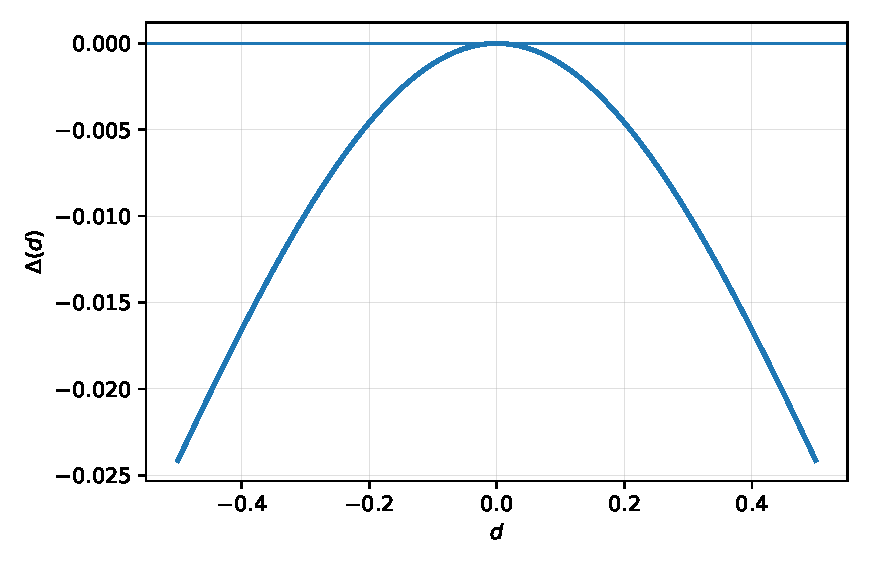
\includegraphics[width=.76\textwidth]{ou_counterexample_defect.pdf}
\caption{Exact counterexample defect for $a_0=3/2$, $\epsilon=2/5$, and $c=9/10$ on the finite rational test domain. The curve is generated from \cref{eq:ou_defect}; it is not fitted data.}
\label{fig:ou_defect}
\end{figure}

\section{Finite exact counterexample certificate}
The executable test uses
\begin{equation}
 a_0=\frac32,
 \qquad
 \epsilon=\frac25,
 \qquad
 c=\frac9{10},
 \label{eq:ou_test_params}
\end{equation}
and evaluates
\begin{equation}
 d=\frac{i}{1000},
 \qquad
 i=-500,\ldots,500.
 \label{eq:ou_test_grid}
\end{equation}
All arithmetic is rational. The domain contains \CRTCCounterGridPoints{} points. The test proves $a(d)>0$ at every point, obtains zero defect at $d=0$, and obtains a strictly negative defect at each of the remaining \CRTCCounterOffCircle{} points.

The finite sweep is a regression check for the explicit family, while \cref{eq:ou_defect} is the continuum proof. In particular, the sign of the defect is known analytically for every real nonzero $d$ when the stated positive parameters are used.

\section{The rigid correlated class is nonempty}
Set $\epsilon=0$ while keeping $a_0>0$ and $b(d)=cd$. The same stochastic construction has
\begin{equation}
 K(d)=a_0I+cdJ,
 \label{eq:ou_rigid_k}
\end{equation}
positive symmetric dissipation, a stationary isotropic covariance, and exact Green Kubo response
\begin{equation}
 Z(d)=\frac1{a_0+icd}.
 \label{eq:ou_rigid_z}
\end{equation}
By \cref{eq:defect_ab}, its defect vanishes identically. Thus the admissible class contains both rigid and nonrigid members. The distinction is not correlation versus no correlation; it is whether the dissipative part of the measured inverse response is flat in chirality.

\section{What can be decided from a spectrum}
In an identified two dimensional shear block of the form $aI+bJ$, the eigenvalues are
\begin{equation}
 q_\pm=a\pm ib.
 \label{eq:shear_spectrum}
\end{equation}
If the response normalization or residue is known so that these eigenvalues are indeed the inverse response coordinates, the circle criterion is immediate: compare their common real part with the achiral value. No time domain simulation is required.

This statement must not be expanded to an arbitrary microscopic spectrum. A Green Kubo coefficient has the schematic resolvent form
\begin{equation}
 \mathcal{R}=\langle g,L^{-1}h\rangle
 \label{eq:resolvent_matrix_element}
\end{equation}
on the nonconserved subspace. Eigenvalues of $L$ matter, but so do eigenvectors, spectral projectors, and the overlaps of the observable and source with those modes.

The CRTC package includes an exact two dimensional witness. Let
\begin{equation}
 L_1=\begin{pmatrix}1&0\\0&2\end{pmatrix},
 \qquad
 S=\begin{pmatrix}1&1\\0&1\end{pmatrix},
 \qquad
 L_2=S L_1S^{-1}.
 \label{eq:same_spectrum_matrices}
\end{equation}
The matrices are similar and therefore have exactly the same spectrum. With fixed $g=(1,0)$ and $h=(0,1)^T$, however,
\begin{equation}
 gL_1^{-1}h\ne gL_2^{-1}h.
 \label{eq:different_overlap}
\end{equation}
The bare unordered full spectrum is therefore insufficient to determine a general response matrix element.

\section{Meaning for collision operators}
The distinction suggests a practical decision tree. If a microscopic analysis isolates the exact shear invariant subspace, identifies its effective generator, and fixes the response residue, then the complex pair can decide CRTC membership algebraically. If additional slow variables mix with shear, or if only the full list of eigenvalues is known, one must project or eliminate the additional variables and compute the actual scalar complex response before applying the theorem.

This is particularly relevant beyond molecular chaos. Correlations can generate a frequency dependent self energy or memory kernel. A two component form may survive symmetry reduction, but its coefficients can depend on frequency, size, and chirality. The classifier remains valid at each fixed prescription:
\begin{equation}
 \RePart\!\left[\frac1{Z_{L,\omega}(p)}\right]
 =\RePart\!\left[\frac1{Z_{L,\omega}(p_0)}\right]
 \label{eq:regulated_classifier}
\end{equation}
if and only if the regulated response lies on its anchored circle.

\section{Chapter conclusion}
The counterexample closes the structural classification at the level that symmetry and positivity can address. There exists a correlated positive dissipation rigid class and a correlated positive dissipation nonrigid class. Consequently $C_6$, reflection parity, stationarity, and positivity do not determine the outcome. An identified reduced shear spectrum can decide membership, while a bare full spectrum generally cannot. The remaining task is therefore model specific: determine the actual correlated inverse shear response of the chiral FHP automaton or prove an identity that constrains it.

\chapter{Discussion: What Would Correlated CRTC Survival Mean?}\label{ch:discussion}

\section{The open physical statement}
The exact theorem of \cref{ch:rigidity} does not settle whether the fully correlated chiral FHP automaton preserves the kinetic circle. It turns that question into a precise condition. Under any stated finite size, finite time, frequency, or running scale prescription, define the actual complex shear response $Z(p)$. Correlated CRTC survival means
\begin{equation}
 \RePart\!\left[\frac1{Z(p)}\right]
 =\RePart\!\left[\frac1{Z(p_0)}\right]
 \label{eq:discussion_survival}
\end{equation}
throughout the chirality domain of interest.

If \cref{eq:discussion_survival} holds, shear and Hall viscosities are not independent functions of chirality under that prescription. One real function, together with the anchor and parity, determines their location on a one dimensional geometric constraint. The response map has fewer independent degrees of freedom than a generic pair of transport functions.

If it fails, the defect formula identifies the cause without ambiguity at the response level: the real part of the measured inverse response has acquired chirality dependence. The theorem does not require one to guess whether the failure came from a collision eigenvalue shift, a response residue, a memory kernel, or coupling to another slow variable. Those are microscopic explanations of a measured inverse response drift, not alternative definitions of the drift.

\section{What survival would say about renormalization}
In the molecular chaos calculation, the complex shear eigenvalue follows a vertical line at fixed density. Correlations can be described formally by an effective inverse response, a memory function, or a self energy. If the reduced shear problem remains two dimensional, correlated CRTC survival requires the renormalized dissipative inverse coordinate to be independent of chirality relative to the achiral anchor.

That is a restrictive statement. Parity allows an expansion
\begin{equation}
 a(d)=a_0+a_2d^2+a_4d^4+\cdots.
 \label{eq:discussion_even_drift}
\end{equation}
Every coefficient after $a_0$ must vanish for exact rigidity. Symmetry does not set them to zero. A proof of survival must therefore identify additional dynamics that forbids all such even chirality corrections or makes their combined contribution cancel in the actual measured inverse response. In particular, this is not a Ward identity established by the present symmetry analysis; such a statement would require an additional microscopic symmetry or conservation law.

The RG criterion \cref{eq:rg_tangent} is one way to express that requirement. If the rigid manifold is preserved by scale evolution, then the flow of the dissipative coordinate must be the same at $p$ and at the anchor whenever the response starts on the manifold. This is stronger than saying that the odd coordinate has a special parity or that odd viscosity is reactive.

\section{Odd viscosity does not by itself protect the circle}
Odd viscosity is nondissipative in the conventional constitutive energy balance \cite{Avron1998,Banerjee2017}. That fact means that the antisymmetric transport component does not directly contribute to entropy production in the same way as ordinary shear viscosity. It does not imply that the dissipative coefficient is immune to chirality dependent correlation corrections.

The counterexample in \cref{ch:counterexample} makes this logical point explicit. The reactive coordinate is odd, the symmetric drift is positive, and the stationary response is exactly computable, yet $a(d)$ drifts and the circle fails. Protection of CRTC therefore requires a statement about the dissipative inverse response, not merely the nondissipative character of $\eta_H$.

Likewise, results concerning topological Hall viscosity in gapped quantum systems should not be transferred automatically to a classical two dimensional lattice gas. The symmetry class, state space, conservation laws, and hydrodynamic fluctuation structure are different.

\section{Long time tails and the order of limits}
The 1990 FHP long time tail calculation shows why the correlated problem should not be phrased only as a single infinite time number \cite{Naitoh1990}. At fixed finite lattice size, a deterministic cellular automaton has a finite state space and ultimately recurrent dynamics. In an infinite hydrodynamic scaling limit, long wavelength modes can generate algebraic tails. A physically meaningful transport statement must specify how these limits are approached.

Useful regulated responses include
\begin{equation}
 Z_{L,T}(p),
 \qquad
 Z_{L}(\omega,p),
 \qquad
 Z_{\ell}(p).
 \label{eq:regulated_responses}
\end{equation}
Here $L$ is system size, $T$ an integration cutoff, $\omega$ a frequency, and $\ell$ a coarse graining scale. The rigidity theorem applies separately to each nonzero regulated response. One can then ask whether the defect remains zero, tends to zero, approaches a nonzero function, or fails to converge as the regulator changes.

A common divergence in both coordinates would not by itself decide the normalized geometry. What matters is the chirality dependence of $\RePart(1/Z)$ at the same regulator. This formulation avoids claiming that a divergent shear viscosity can simply be subtracted away while preserving a finite odd coordinate.

\section{A falsification path}
The theorem gives a direct falsification strategy for any future exact or numerical correlated calculation.

\begin{enumerate}[label=\arabic*.]
\item Fix density, boundary conditions, ensemble, system size, response frequency or integration window, and the definition of the shear observables.
\item Compute or estimate the complex response $Z(p)$ and the achiral anchor $Z(p_0)$ under the same prescription.
\item Form the inverse response and measure
\begin{equation}
 G(p)=\RePart[1/Z(p)]-\RePart[1/Z(p_0)].
 \label{eq:falsification_g}
\end{equation}
\item Test whether $G(p)$ is identically zero within exact arithmetic or whether its uncertainty interval excludes zero in a controlled statistical calculation.
\item If $G$ is nonzero, use the defect identity to predict the corresponding circle departure and compare it with the directly measured geometric defect.
\item Repeat the analysis while changing the regulator to distinguish a finite scale effect from a stable asymptotic trend.
\end{enumerate}

A circle fit alone is weaker than this procedure. A finite set of noisy points can look circular even when inverse dissipative drift is present, and many circles can fit a short arc. The anchored inverse response criterion tests the specific relation derived from the parity anchor.

\section{What would count as a proof}
A model specific proof of correlated CRTC survival could take several forms.

One route would be an exact microscopic identity showing that the chirality dependent contribution to $\RePart(1/Z)$ vanishes. Such an identity could arise from a previously unrecognized conservation law or exact decoupling of the dissipative shear channel.

A second route would be a controlled renormalization calculation proving that the rigid manifold is invariant, that is, deriving \cref{eq:rg_tangent} from the microscopic model at every relevant scale.

A third route would be an exact finite system resolvent calculation followed by a mathematically controlled limiting argument. In that case the response residue and mode overlaps must be retained; the unordered spectrum alone is not sufficient.

A fourth route could use another nonperturbative construction that computes the same response and proves the invariant directly. The structural theorem is agnostic about which route is used. What matters is that the actual correlated $Z$ satisfies \cref{eq:discussion_survival}.

\section{Comparison with familiar transport relations}
Relations such as Wiedemann Franz or Stokes Einstein link distinct transport quantities under particular physical assumptions. CRTC, if established for a correlated microscopic model, would likewise reduce independent transport data. The comparison should remain conceptual rather than literal. Those relations have their own conservation laws, quasiparticle assumptions, or fluctuation mechanisms. The present theorem does not derive them and does not borrow their protection arguments.

The Kramers Kronig analogy is even more limited. Kramers Kronig relations use analyticity in frequency and causality to link dispersive and absorptive response components. CRTC instead concerns the path of a static or fixed prescription response as a chirality control parameter changes. Both use complex response notation, but the independent variable and mathematical reason for the relation are different.

\section{Potential generalization}
The closure free theorem is not tied to FHP. Any two component response with a real positive anchor can be tested by \cref{eq:rig_theorem}. The $C_6$ commutant calculation is more specific: it explains why a hexagonal shear sector reduces naturally to a complex scalar. Other point groups can produce different commutants and therefore different response geometries.

A useful general program is to classify response manifolds by three ingredients: the symmetry commutant of the relevant tensor sector, the analytic map from the effective kernel to the measured response, and the invariant submanifolds of the renormalization flow. In the present case those ingredients are a complex scalar commutant, inversion, and the vertical line $\RePart Q=a_0$. The image is a circle. In a higher dimensional or anisotropic sector, the corresponding geometry need not be circular.

\section{Limits of the current evidence}
The repository includes preserved external numerical traces with incomplete provenance. They are not used to support the correlated CRTC claim. No generator, units, ensemble, lattice size, integration time, or estimator is documented well enough to turn those values into evidence for a Green Kubo limit. Retaining the files while excluding them from proof is preferable to assigning semantics that the record does not contain.

The current exact endpoint automaton is also not the complete continuous chiral FHP family. A future study that mixes endpoint rules stochastically or implements the published $p$ dependent collisions must document that model independently and should not describe the endpoint exhaustive certificate as an exhaustive test over $p$.

Finally, the Ornstein Uhlenbeck model is a counterexample to structural protection by symmetry and positivity. It is not evidence that the chiral FHP automaton breaks the circle. Its role is to show that a model specific argument is logically necessary.

\section{Chapter conclusion}
If correlated CRTC survival is eventually proved, its meaning is precise: the dissipative part of the measured inverse shear response remains chirality independent under the specified response prescription, so shear and Hall viscosities occupy one constrained response manifold rather than two independent functions. The present work establishes the classifier and the obstruction class, not the missing microscopic protection theorem. This distinction turns a visual pattern into a falsifiable structural question.

\chapter{Conclusion and Outlook}\label{ch:conclusion}

\section{What is established}
This thesis develops a hierarchy from exact microscopic maps to a closure free response classification.

At the microscopic level, the deterministic six channel endpoint gas has an exact collision dressed reversor. The identities $\Theta_\chi^2=I$ and $\Theta_\chi F_\chi\Theta_\chi=F_\chi^{-1}$ imply an all time echo on every finite periodic torus under the stated definitions. The implementation is supported by an exhaustive \HXGlobalStates{} state certificate on the complete $2\times2$ torus for both chiralities and an independent oracle on larger tori. The local collision table has a three dimensional space of one body linear invariants generated by mass and the two momentum components.

At the kinetic level, the published chiral FHP coefficients of Allocca \etal\ obey an exact circle after the lattice shear shift is included. Their complex response is the inverse of the conjugate shear eigenvalue up to a fixed numerical factor, and the kinetic circle is the image of a vertical eigenvalue locus under complex inversion. Independent exact arithmetic checks reproduce these identities over two distinct declared grids.

At the structural level, the central theorem is independent of that kinetic closure. For any nonzero complex response with a positive real achiral anchor, membership in the anchored circle is equivalent to constancy of the real part of the inverse response. In coordinates $1/Z=a+ib$, the defect is exactly \cref{eq:defect_ab}. The theorem is both necessary and sufficient for this circle membership predicate.

The $C_6$ shear commutant is exactly two dimensional and has form $aI+bJ$. Reflection makes $a$ even and $b$ odd in chirality displacement, but neither symmetry forces $a$ to remain constant. The achiral curvature formula identifies quadratic dissipative drift, while a quartic drift example proves that local curvature at one point does not decide global circle membership.

Finally, a stable stationary Ornstein Uhlenbeck model provides an exact correlated Green Kubo witness with positive dissipation that leaves the circle whenever $a(d)$ drifts. The rigid family obtained by constant $a$ is equally admissible. Symmetry, stationarity, and positivity therefore permit both classes.

\section{What remains open}
The fully correlated chiral FHP question remains open. The thesis does not prove that the effective Green Kubo response of that model has constant inverse dissipative coordinate. It also does not prove that the circle fails. What it supplies is the exact condition that either result must satisfy.

The strongest next step is not a larger unconstrained circle fit. It is a derivation or controlled computation of
\begin{equation}
 G_{L,\omega}(p)=
 \RePart\!\left[\frac1{Z_{L,\omega}(p)}\right]
 -\RePart\!\left[\frac1{Z_{L,\omega}(p_0)}\right]
 \label{eq:conclusion_g}
\end{equation}
with all regulators and observables specified. An exact zero would support rigidity at that prescription. A reproducible nonzero value would falsify it there. The behavior under size, frequency, and time scaling would then decide whether the effect persists in a hydrodynamic limit.

A more ambitious route is to seek a microscopic identity or RG argument that enforces \cref{eq:rg_tangent}. Such a result would supply the missing protection principle. Only at that point would Ward identity language be justified.

\section{Broader implication}
The main conceptual outcome is a method for separating response geometry from the approximation that first revealed it. A circle seen in a kinetic theory need not be treated as a fragile numerical curiosity, nor should it be assumed universal. By moving to the measured inverse response, one can identify the exact invariant, determine which symmetry restrictions are automatic, and construct counterexamples that isolate what remains to be proved.

That method extends beyond the specific lattice gas. Whenever symmetry reduces a transport sector to a low dimensional commutant, the response map can be studied as the image of that effective kernel under the measurement map. Fixed submanifolds in kernel space then become geometric constraints in response space. The scientific task is to prove which of those submanifolds are dynamically preserved.

\section{Final statement}
The chiral transport circle is exact in the published molecular chaos formulas. The response rigidity theorem states exactly what it would mean for the circle to survive beyond that closure. The counterexample proves that survival is not guaranteed by the obvious symmetry and positivity assumptions. The remaining correlated FHP problem is therefore well posed: determine whether its actual inverse shear response stays on the rigid manifold under a controlled Green Kubo or renormalized response prescription.


\appendix
\chapter{Proof Details}\label{app:proofs}

\section{Anchored circle and inverse response}
Let $Z=x+iy\ne0$ and let $Z_0=x_0>0$. The circle with diameter $[0,x_0]$ is
\begin{equation}
 \left(x-\frac{x_0}{2}\right)^2+y^2=\left(\frac{x_0}{2}\right)^2.
 \label{eq:app_circle}
\end{equation}
Expansion gives
\begin{equation}
 x^2+y^2-x_0x=0.
 \label{eq:app_delta_zero}
\end{equation}
Since
\begin{equation}
 \frac1Z=\frac{x-iy}{x^2+y^2},
 \label{eq:app_inverse}
\end{equation}
we have
\begin{equation}
 \RePart\!\left(\frac1Z\right)=\frac{x}{x^2+y^2}.
 \label{eq:app_inverse_real}
\end{equation}
Therefore \cref{eq:app_delta_zero} is equivalent to
\begin{equation}
 1=x_0\RePart\!\left(\frac1Z\right).
 \label{eq:app_classifier}
\end{equation}
At the anchor, $1/Z_0=1/x_0$, completing the proof of \cref{eq:rig_theorem}.

If $1/Z=a+ib$, then $x=a/(a^2+b^2)$ and $|Z|^2=1/(a^2+b^2)$. With $x_0=1/a_0$,
\begin{align}
 \Delta
 &=\frac1{a^2+b^2}
 -\frac1{a_0}\frac{a}{a^2+b^2}\\
 &=\frac{a_0-a}{a_0(a^2+b^2)},
\end{align}
which is \cref{eq:defect_ab}.

\section{Commutant of the shear representation}
For the $120$ degree shear representation matrix
\begin{equation}
 R=\begin{pmatrix}
 -1/2&-\sqrt3/2\\
 \sqrt3/2&-1/2
 \end{pmatrix}
\end{equation}
and a generic real matrix
\begin{equation}
 M=\begin{pmatrix}r&s\\t&u\end{pmatrix},
\end{equation}
the equation $MR-RM=0$ has two independent scalar constraints:
\begin{equation}
 r-u=0,
 \qquad
 s+t=0.
\end{equation}
Thus $M=rI-sJ$ with $J^2=-I$. The independent symbolic audit obtains the same solution with no import from the project response code.

\section{Curvature at the parity anchor}
Write
\begin{equation}
 a(d)=a_0+\frac12a_2d^2+O(d^4),
 \qquad
 b(d)=b_1d+O(d^3),
\end{equation}
and
\begin{equation}
 Z(d)=\frac{a(d)-ib(d)}{a(d)^2+b(d)^2}.
\end{equation}
Parity implies $x'(0)=0$ and $y''(0)=0$. Direct differentiation gives
\begin{equation}
 y'(0)=-\frac{b_1}{a_0^2}
\end{equation}
and
\begin{equation}
 x''(0)=-\frac{a_2}{a_0^2}-\frac{2b_1^2}{a_0^3}.
\end{equation}
Using the signed curvature definition \cref{eq:curvature_general},
\begin{equation}
 \kappa(0)=
 \frac{-y'(0)x''(0)}{|y'(0)|^3}.
\end{equation}
For $b_1>0$, this reduces to
\begin{equation}
 \kappa(0)=-2a_0-\frac{a_0^2a_2}{b_1^2}.
\end{equation}
Changing the orientation changes the overall sign, not the magnitude of the curvature or the dependence on $a_2$.

\section{Quartic drift witness}
For $a(d)=a_0+\epsilon d^4$ and $b(d)=cd$, the second derivative $a''(0)$ vanishes, so the achiral curvature equals the rigid circle value. The exact defect is nevertheless
\begin{equation}
 \Delta(d)=
 -\frac{\epsilon d^4}
 {a_0[(a_0+\epsilon d^4)^2+c^2d^2]}.
\end{equation}
For $a_0>0$, $\epsilon\ne0$, and any nonzero $d$ for which the denominator is finite, the defect is nonzero. This proves that achiral curvature is not a complete global membership test.

\section{Published kinetic circle}
With $x=A/(1+u^2)$ and $y=-Au/(1+u^2)$,
\begin{equation}
 x^2+y^2
 =\frac{A^2+A^2u^2}{(1+u^2)^2}
 =\frac{A^2}{1+u^2}=Ax.
\end{equation}
The kinetic circle follows without approximation after the published coefficients are accepted as the starting expressions.

For the eigenvalue
\begin{equation}
 \lambda=-\frac{D}{2}+i\frac{\sqrt3D}{3}d,
\end{equation}
we have
\begin{align}
 -\frac1{4\lambda^*}
 &=\frac{1}{2D}\frac{1-i(2\sqrt3/3)d}{1+(4/3)d^2}\\
 &=\bar\eta+i\eta_H,
\end{align}
which proves the spectral relation used by the exact test.

\section{OU stationary covariance and Green Kubo integral}
For $K=aI+bJ$ and $C=AI$,
\begin{align}
 KC+CK^T
 &=A(aI+bJ)+A(aI-bJ)\\
 &=2AaI.
\end{align}
If $a>0$, this covariance is positive definite. Since the eigenvalues $a\pm ib$ have positive real part,
\begin{equation}
 \int_0^\infty \e^{-Kt}\,\dd t=K^{-1}.
\end{equation}
Multiplying by $C$ yields \cref{eq:ou_gk}. No numerical quadrature is needed.

\section{Same spectrum, different response matrix element}
Similarity preserves the characteristic polynomial, so the matrices $L_1$ and $L_2$ in \cref{eq:same_spectrum_matrices} have identical eigenvalues. Explicitly,
\begin{equation}
 L_2=\begin{pmatrix}1&1\\0&2\end{pmatrix},
 \qquad
 L_2^{-1}=\begin{pmatrix}1&-1/2\\0&1/2\end{pmatrix}.
\end{equation}
For $g=(1,0)$ and $h=(0,1)^T$,
\begin{equation}
 gL_1^{-1}h=0,
 \qquad
 gL_2^{-1}h=-\frac12.
\end{equation}
Thus an unordered eigenvalue list cannot determine the resolvent matrix element without overlap information.

\chapter{Machine and Executable Definitions}\label{app:machine}

\section{Purpose}
This appendix records the executable objects that support the thesis. It is not a substitute for the source files. Paths are given so that each statement can be traced to the canonical implementation.

\begin{longtable}{p{.32\textwidth}p{.58\textwidth}}
\toprule
Path & Role \\
\midrule
\endhead
\texttt{src/chiral\_law.c} & Standalone deterministic chiral gas certificate, including local collision permutations, streaming, reflection, velocity reversal, exhaustive $2\times2$ state enumeration, echo, and correlation witness.\\
\texttt{tests/test\_chiral\_law.py} & Independent Python oracle for larger tori, multiple echo times, collision covariance, and exact rational one body invariant rank.\\
\texttt{tests/test\_transport\_circle.py} & Exact $\mathbb{Q}(\sqrt3)$ reconstruction of the published kinetic transport circle, spectral relation, and weak field image.\\
\texttt{research/crtc/src/crtc} & Response geometry, FHP reconstruction, correlated models, spectral tests, renormalization criterion, and numerical monitor.\\
\texttt{research/crtc/tests} & Thirty five unit tests including symbolic identities and finite exact domains.\\
\texttt{polyforms/entropy.hx} & Five dimensional sparse Polyform with explicit termination cells on all ten signed entropy exits.\\
\texttt{tests/test\_entropy\_sparse.py} & Regression for seed $12345$ and complete signed axis endpoint coverage.\\
\texttt{evidence} & Regenerated machine certificates, waveforms, images, state snapshots, and release evidence.\\
\bottomrule
\end{longtable}

\section{Sparse field termination}
The entropy Polyform uses rows of the form
\begin{center}
\texttt{CELL x y z w v opcode arg0 arg1 arg2}.
\end{center}
The origin executes the entropy selector. Each first step cell emits one axis letter. Each signed distance two endpoint has opcode zero, which is the explicit HALT operation in this Polyform encoding. All ten endpoints are present. This representation preserves the semantic distinction between an intentional halt and execution into an undefined sparse coordinate.

\section{Build products and evidence}
The root Makefile builds the x86\_64 HX89 executable, the HX0 bootstrap, the pulse PCM signal tool, the hex gas, the byte Polyform tool, and the chiral proof executable. Release evidence regenerates canonical machine outputs rather than shipping only a handwritten report.

The thesis itself is added as another reproducible target. Its generated values come from existing evidence and test definitions, while its independent symbolic audit is intentionally outside the CRTC import path.

\section{External data boundary}
Files under \texttt{evidence/external\_runs/raw} are retained verbatim when present. Their metadata is insufficient for scientific use. They are not parsed into plots, not included in numerical claims, and not used as input to any theorem test in this thesis. This rule prevents accidental promotion of unknown traces into evidence.

\chapter{Reproducibility Manifest}\label{app:repro}

\section{Primary command}
From the repository root, the complete verification target is
\begin{lstlisting}
make verify-all
\end{lstlisting}
The target runs the machine suite, sanitizer checks, CRTC verification, independent thesis mathematics audit, generated fragment consistency, prose lint, thesis compilation, companion compilation, and document consistency checks. The release audit remains available separately when a full evidence regeneration is desired.

\section{Expected scientific certificates}
A valid run must include the following logical outcomes:
\begin{enumerate}[label=\arabic*.]
\item the HX89 runtime suite reports all tests passed;
\item the entropy regression reports seed $12345$ passed and all ten signed five axis exits terminate explicitly;
\item the chiral law certificate reports \HXLocalStates{} local states and \HXGlobalStates{} global states with mirror chirality, involution, reversor, echo, and correlation reciprocity passing;
\item the transport certificate reports \HXTransportGridPoints{} exact rational $(\rho,p,B)$ points in $\mathbb{Q}(\sqrt3)$;
\item the CRTC module reports \CRTCUnitTests{} passing tests, including \CRTCBoltzmannGridPoints{} exact Boltzmann grid points and \CRTCCounterGridPoints{} counterexample grid points;
\item the independent symbolic audit reports every listed derivation passed;
\item the LaTeX log contains no undefined references or citations.
\end{enumerate}

\section{Generated thesis fragments}
The file \texttt{generated/canonical.tex} is not edited by hand. It is regenerated by
\begin{lstlisting}
python3 thesis/tools/generate_fragments.py
\end{lstlisting}
and checked by
\begin{lstlisting}
python3 thesis/tools/generate_fragments.py --check
\end{lstlisting}
The generator reads the certificates and executable test domains. If a domain changes, the thesis cannot pass the stale fragment check until the generated values are rebuilt.

\section{Independent symbolic audit}
The command
\begin{lstlisting}
python3 thesis/tools/independent_math_audit.py
\end{lstlisting}
uses SymPy but imports no package from \texttt{research/crtc/src}. It independently checks the response defect, commutant, kinetic circle, spectral inversion, curvature expression, quartic witness, OU Green Kubo construction, and spectral overlap obstruction.

\section{Document build}
The document build uses \texttt{latexmk}, BibTeX, and the glossary tool. Equation numbers and cross references are semantic LaTeX labels. The consistency checker scans the final logs for unresolved citations or references and confirms that all generated macros are current.

The two compiled documents are:
\begin{itemize}
\item \texttt{thesis/Alex\_Moraru\_Thesis.pdf};
\item \texttt{thesis/Alex\_Moraru\_Thesis\_Companion.pdf}.
\end{itemize}
Their TeX sources, bibliography, glossary definitions, figures, and generation scripts are included in the same repository.

\section{Manifest policy}
After every verification and document build, the repository manifest is regenerated from the final file tree. Transient LaTeX auxiliary files and Python caches are removed from the distributable tree. Compiled PDFs and human readable verification transcripts are retained. The external ZIP checksum is reported separately at handoff so that it cannot be self referential.

\chapter{Scope, Novelty Boundary, and Anticipated Objections}\label{app:adversarial}

\section{Objection one: the circle is only complex inversion}
\textbf{Strong form of the objection.} Complex inversion maps a vertical line to a circle. Semicircular complex response plots are classical. Therefore the transport circle is a change of coordinates rather than a substantive result.

\textbf{Response.} The geometric fact is classical and is not claimed as new. The substantive result is the exact classification of the anchored chiral response condition in terms of the measured inverse response, together with the symmetry boundary and the explicit correlated counterexample. In the published chiral FHP kinetic theory, the circle is indeed the inverse image of a vertical shear eigenvalue line. Beyond that closure, the theorem identifies exactly what must remain vertical after all residues, projections, and correlation effects are included in the measured response.

\textbf{Boundary of the defense.} The theorem does not establish a new general theorem about Mobius transformations. Its physical value depends on whether the inverse response criterion clarifies and constrains the correlated chiral transport problem.

\section{Objection two: $C_6$ symmetry should already force the result}
\textbf{Strong form of the objection.} Hexagonal isotropy reduces the shear sector to two scalar coefficients, so the circle may be only a symmetry consequence.

\textbf{Response.} The commutant calculation proves the opposite. $C_6$ permits every matrix $aI+bJ$. Reflection makes $a$ even and $b$ odd in chirality displacement, but allows arbitrary even drift in $a$. The positive dissipation OU family chooses $a=a_0+\epsilon d^2$ and $b=cd$ and obeys the same symmetry form while violating the circle exactly. Symmetry explains the two coordinate complex structure, not dissipative flatness.

\textbf{Boundary of the defense.} A stronger microscopic symmetry or conservation law could still force $a$ to remain constant in a particular model. The thesis has not found or proved such a law for correlated chiral FHP.

\section{Objection three: the counterexample is not FHP}
\textbf{Strong form of the objection.} An Ornstein Uhlenbeck process is too simple and is not a cellular automaton, so it cannot decide whether the FHP circle survives correlations.

\textbf{Response.} It is not intended to decide the FHP outcome. It answers a different logical question: whether stationarity, positive dissipation, reflection covariance, and the two component rotational normal form are sufficient to protect the circle. The exact counterexample shows that they are not. Consequently any proof for chiral FHP must use additional model specific structure.

\textbf{Boundary of the defense.} The counterexample cannot be used as evidence that correlated FHP breaks the circle. It only proves that the broad structural assumptions do not determine the answer.

\section{Why this model rather than a direct Green Kubo simulation?}
A direct simulation would provide finite regulator evidence but would not by itself establish the structural necessity or sufficiency of circle preservation. The inverse response theorem answers that structural question exactly. Simulation remains valuable as a later model specific test of $G_{L,T}(p)$ or $G_L(\omega,p)$.

\section{Why the parity anchored circle?}
The parity symmetric point supplies a distinguished real response value because the Hall coordinate vanishes there under the stated reflection symmetry. The circle with diameter between zero and this anchor is exactly the image of the vertical inverse response line through $a_0$. Other circles can be considered, but they represent different geometric constraints and are not CRTC as defined here.

\section{Why not classify only by curvature?}
Curvature is local. The quartic drift witness has the same achiral curvature as the rigid circle but leaves it away from the anchor. A global classifier must therefore use the inverse response identity or an equivalent condition over the domain.

\section{Prior art challenge}
\textbf{Question.} Is this only the 2026 chiral FHP result rewritten in complex notation?

\textbf{Answer.} The published work supplies the kinetic coefficients and the chiral lattice gas setting \cite{Allocca2026}. The present structural theorem does not assume those coefficients. It applies to any nonzero measured complex response and remains valid if correlations renormalize both the effective kernel and the response residue. The counterexample and spectral overlap obstruction also lie outside the published kinetic derivation. Conversely, the thesis attributes the molecular chaos coefficients and does not claim their derivation as original.

\section{Overclaim audit of the abstract}
\begin{longtable}{p{.42\textwidth}p{.48\textwidth}}
\toprule
Abstract statement & Support and boundary \\
\midrule
\endhead
Deterministic endpoint reciprocity is exact. & Operator identities plus exhaustive finite implementation certificate and independent oracle. Does not imply a viscosity value.\\
Published Boltzmann coefficients lie on a circle. & Algebraic elimination of cited formulas plus exact rational tests. Conditional on the published molecular chaos theory.\\
Anchored circle membership is equivalent to constant $\RePart(1/Z)$. & Exact algebraic theorem for every nonzero response with stated anchor.\\
$C_6$ gives $aI+bJ$ but not constant $a$. & Exact commutant solution plus explicit symmetry allowed drift.\\
A positive dissipation correlated counterexample exists. & Exact OU Lyapunov and Green Kubo calculation plus rational grid test. Not an FHP surrogate.\\
Correlated FHP survival remains open. & No current repository proof establishes the required constant inverse real part under a correlated response prescription.\\
\bottomrule
\end{longtable}

\section{Defense questions}
The following questions should be answerable directly from the thesis and repository.
\begin{enumerate}[label=\arabic*.]
\item Where exactly does molecular chaos enter the circle result?
\item Which statement is proved by $C_6$ symmetry, and which statement is not?
\item Why is $\RePart(1/Z)$ preferred to a bare collision eigenvalue when a response residue can vary?
\item What role do long time tails play in defining the correlated question?
\item Why is local curvature insufficient for the global classification?
\item What additional data beyond eigenvalues are needed for a general Green Kubo resolvent matrix element?
\item Which result would have to be proved before Ward identity language becomes justified?
\item What, precisely, does the OU counterexample falsify and what does it not falsify?
\end{enumerate}

\chapter{Claim and Evidence Matrix}\label{app:claims}

\begin{longtable}{p{.42\textwidth}p{.18\textwidth}p{.30\textwidth}}
\toprule
Claim & Status & Evidence or limitation \\
\midrule
\endhead
Endpoint collision dressed reversor and all time echo & Proved & Operator composition; C certificate and independent Python oracle verify implementations.\\
One body local collision invariant space has dimension three & Proved & Exact rational elimination in independent oracle.\\
Published chiral FHP molecular chaos coefficients lie on the stated circle & Exact corollary of cited model & Algebraic elimination; \HXTransportGridPoints{} exact $(\rho,p,B)$ checks and separate \CRTCBoltzmannGridPoints{} point zero field check.\\
Anchored circle is equivalent to constant $\RePart(1/Z)$ & Proved & Algebraic identity \cref{eq:rig_master_identity}; independent SymPy audit.\\
For $1/Z=a+ib$, defect equals \cref{eq:defect_ab} & Proved & Direct substitution; two independent symbolic implementations.\\
$C_6$ shear covariance implies $aI+bJ$ & Proved & Exact commutant calculation.\\
$C_6$ forces chirality independent $a$ & False & Even drift $a(d)$ is symmetry allowed; OU witness.\\
Quadratic dissipative drift changes achiral curvature & Proved & Exact curvature formula \cref{eq:curvature_achiral}.\\
Achiral curvature alone decides global membership & False & Quartic drift witness \cref{eq:quartic_drift,eq:quartic_defect}.\\
Positive dissipation and reflection covariance protect CRTC & False & Exact stationary OU counterexample.\\
Rigid positive dissipation correlated class is nonempty & Proved by construction & OU family with constant $a$.\\
Nonrigid positive dissipation correlated class is nonempty & Proved by construction & OU family with $a=a_0+\epsilon d^2$.\\
Identified two dimensional shear spectrum can decide CRTC & Conditional theorem & Requires known response normalization or residue and exact reduced shear block.\\
Bare unordered full spectrum decides a general Green Kubo response & False & Same spectrum different resolvent overlap witness.\\
Defect identity is a Ward identity & Not established & No symmetry or conservation law is proved to enforce rigid flow.\\
Fully correlated chiral FHP preserves CRTC & Open & Requires exact microscopic identity, controlled RG, exact resolvent, or equivalent correlated response derivation.\\
External raw CSV traces support CRTC & Unsupported & Missing generator and schema metadata; excluded from proof.\\
\bottomrule
\end{longtable}


\printglossary[title=Glossary]
\bibliographystyle{unsrtnat}
\bibliography{references}
\end{document}
